\chapter{EVALUACION Y RESULTADOS}
\section{Especificaciones de la prueba}
Con los conjuntos y pares de archivos, se realizo la comparación del algoritmo SCAM frente a los algoritmos Greedy-String-Tiling y Winnowing-Fingerprint. El propósito de las pruebas es obtener los resultados sobre el desempeño de los algoritmos, en términos de precisión y tiempo de ejecución en la deteccion de similitud. En la figura \ref{espePrueba} se ilustra el proceso de las pruebas.


\begin{figure}[!h]
\centering
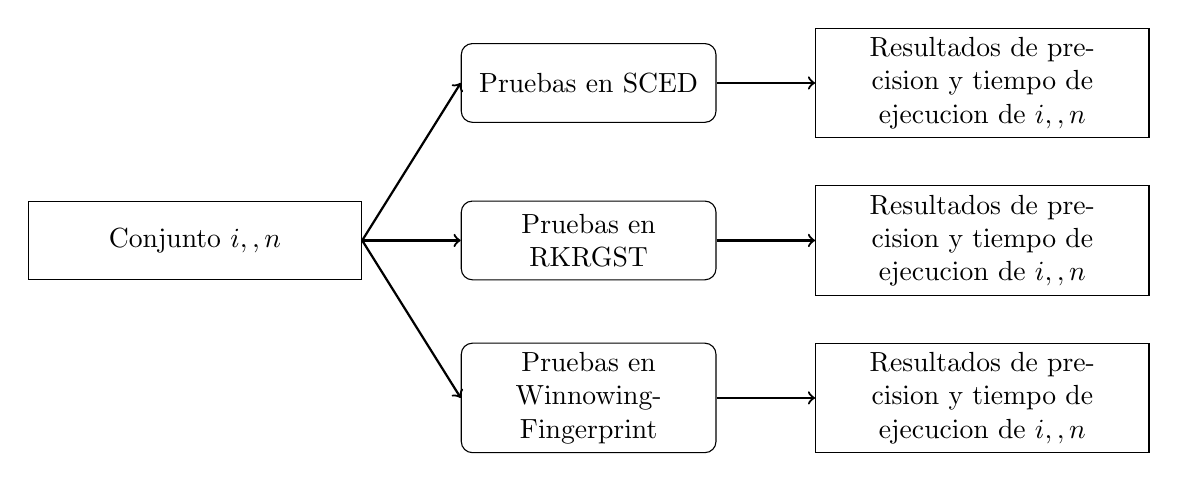
\begin{tikzpicture}[scale=1,
input_output/.style ={rectangle, minimum width=1cm, minimum height=1cm,text centered, text width=4cm, draw=black},
algorithm/.style={rectangle, rounded corners, minimum width=3cm, minimum height=1cm,text centered, text width=3cm, draw=black},
arrow/.style={thick,->,},
]
\node[input_output] (n0) at (1,3) {Conjunto $i, \twodots, n$};
\node[algorithm] (n1) at (6,1) {Pruebas en Winnowing-Fingerprint};
\node[algorithm] (n2) at (6,3) {Pruebas en RKRGST};
\node[algorithm] (n3) at (6,5) {Pruebas en SCED};
\node[input_output] (n4) at (11,1) {Resultados de precision y tiempo de ejecucion de $i, \twodots, n$};
\node[input_output] (n5) at (11,3) {Resultados de precision y tiempo de ejecucion de $i, \twodots, n$};
\node[input_output] (n6) at (11,5) {Resultados de precision y tiempo de ejecucion de $i, \twodots, n$};
\draw [arrow] (n0.east) to (n1.west);
\draw [arrow] (n0.east) to (n2.west);
\draw [arrow] (n0.east) to (n3.west);
\draw [arrow] (n1.east) to (n4);
\draw [arrow] (n2.east) to (n5);
\draw [arrow] (n3.east) to (n6);
\end{tikzpicture}
\caption{Especificacion de las pruebas}
Fuente: Elaboración propia.
\label{espePrueba}
\end{figure}


\subsection{Pruebas de precisión en la deteccion de similitud}
En estas prueba se midió la precisión del algoritmo SCAM frente a los algoritmos Greedy-String-Tiling y Winnowing-Fingerprint. Para cada para de archivos de un conjunto, se realizó la prueba en complejidad temporal de $O(N^2)$. Es decir para un conjunto, se realizó la comparacion de cada par de archivos del mismo.

La precisión de los algoritmos se determino mediante el porcentaje del indice de similitud entre dos archivos. Los resultados obtenidos de la comparacion de similitud entre archivos del conjunto se almacenó en una matriz, y con escala de grises se observó la similitud que existe. Donde los tonos oscuros representan que existe similitud entre dos archivos y los tonos claros representan lo contrario.

\subsection{Tiempo de ejecucion de las pruebas}
Con bibliotecas propias del lenguaje de programacion Python se midio el tiempo de ejecucion de los algoritmos al calcular la similitud en los conjuntos de archivos. La biblioteca utilizada para la medicion fue \id{timeit}. Un ejemplo para la medicion del tiempo de ejecucion de un programa se muestra en el programa \ref{lst:time_it}.

\lstinputlisting[caption={time-it},label={lst:time_it}, language=Python]{programs/time_it.py}

\section{Primera prueba}
En la primera se utilizo los archivos de codigo fuente que se utilizaron en los ejemplos de ofuscacion que se presentó en el marco teorico. En la tabla \ref{firstTest} se muestra el detalle de los programas, el identificador del par y las etiquetas de los programas.

\begin{table}[H]
\centering
\begin{tabular}{|c||c||c|}
\hline
Conjunto & Original & Ofuscado \\ \hline
1 & Programa \ref{lst:obfuscation1_1} & Programa \ref{lst:obfuscation1_2} \\ \hline
2 & Programa \ref{lst:obfuscation2_1} & Programa \ref{lst:obfuscation2_2} \\ \hline
3 & Programa \ref{lst:obfuscation3_1} & Programa \ref{lst:obfuscation3_2} \\ \hline
4 & Programa \ref{lst:obfuscation4_1} & Programa \ref{lst:obfuscation4_2} \\ \hline
5 & Programa \ref{lst:obfuscation5_1} & Programa \ref{lst:obfuscation5_2} \\ \hline
6 & Programa \ref{lst:obfuscation6_1} & Programa \ref{lst:obfuscation6_2} \\ \hline
7 & Programa \ref{lst:obfuscation7_1} & Programa \ref{lst:obfuscation7_2} \\ \hline
8 & Programa \ref{lst:obfuscation8_1} & Programa \ref{lst:obfuscation8_2} \\ \hline
\end{tabular}
\caption{Detalle de los conjuntos de programas con ofuscacion.}
Fuente: Elaboración propia.
\label{firstTest}
\end{table}


\section{Segunda prueba}
En la segunda prueba se utilizo archivos de código fuente en Python enviados por usuarios de un juez de programación. En el cuadro \ref{conjuntoArchivos} se muestra el identificador del conjunto, el numero de problema en el juez, el numero de archivos del conjunto, el promedio de lineas de codigo de los archivos y la varianza de lineas de codigo de los archivos.

\begin{table}[H]
\centering
\begin{tabular}{|c||c|c|c|c|}
\hline
Conjunto & Nro. de Prob. & Nro. de archivos & Prom. de lineas & Var. de lineas \\ \hline \hline
A & 1275  & 10 & 24.8 & 70.84\\ \hline
B & 1407  & 25 & 13.8 & 8.92 \\ \hline
C & 1588  & 41 & 14.24 & 39.84 \\ \hline
D & 1222  & 76 & 2.59 & 0.64 \\ \hline
E & 1089  & 101 & 13.95 & 22.15 \\ \hline
\end{tabular}
\caption{Detalle de los conjuntos de archivos de código fuente para las pruebas}
Fuente: Elaboración propia.
\label{conjuntoArchivos}
\end{table}


\subsection{Prueba de precision I}
En la prueba de precision I, se midió la precision de los algoritmos con un umbral de similitud del $10\%$. Los parametros que utilizaron en los algoritmos fueron los siguientes:
\begin{itemize}
  \item SCBM, $\id{threshold} = 10$
  \item Greedy-String-Tiling, $\id{threshold} = 10$
  \item Winnowing-Fingerprint, $\id{window-length} = 10, \id{k-grams} = 1$
\end{itemize}

\subsubsection{Conjunto A}
La matriz de similitud que se obtuvo para este conjunto de prueba. En la figura \ref{set_A_precision} muestra poca diferencia respecto a la precisión de los algoritmos.
\begin{figure}[!h]
\centering
\subfloat[SCBM]{
\label{SCBM_set_A}
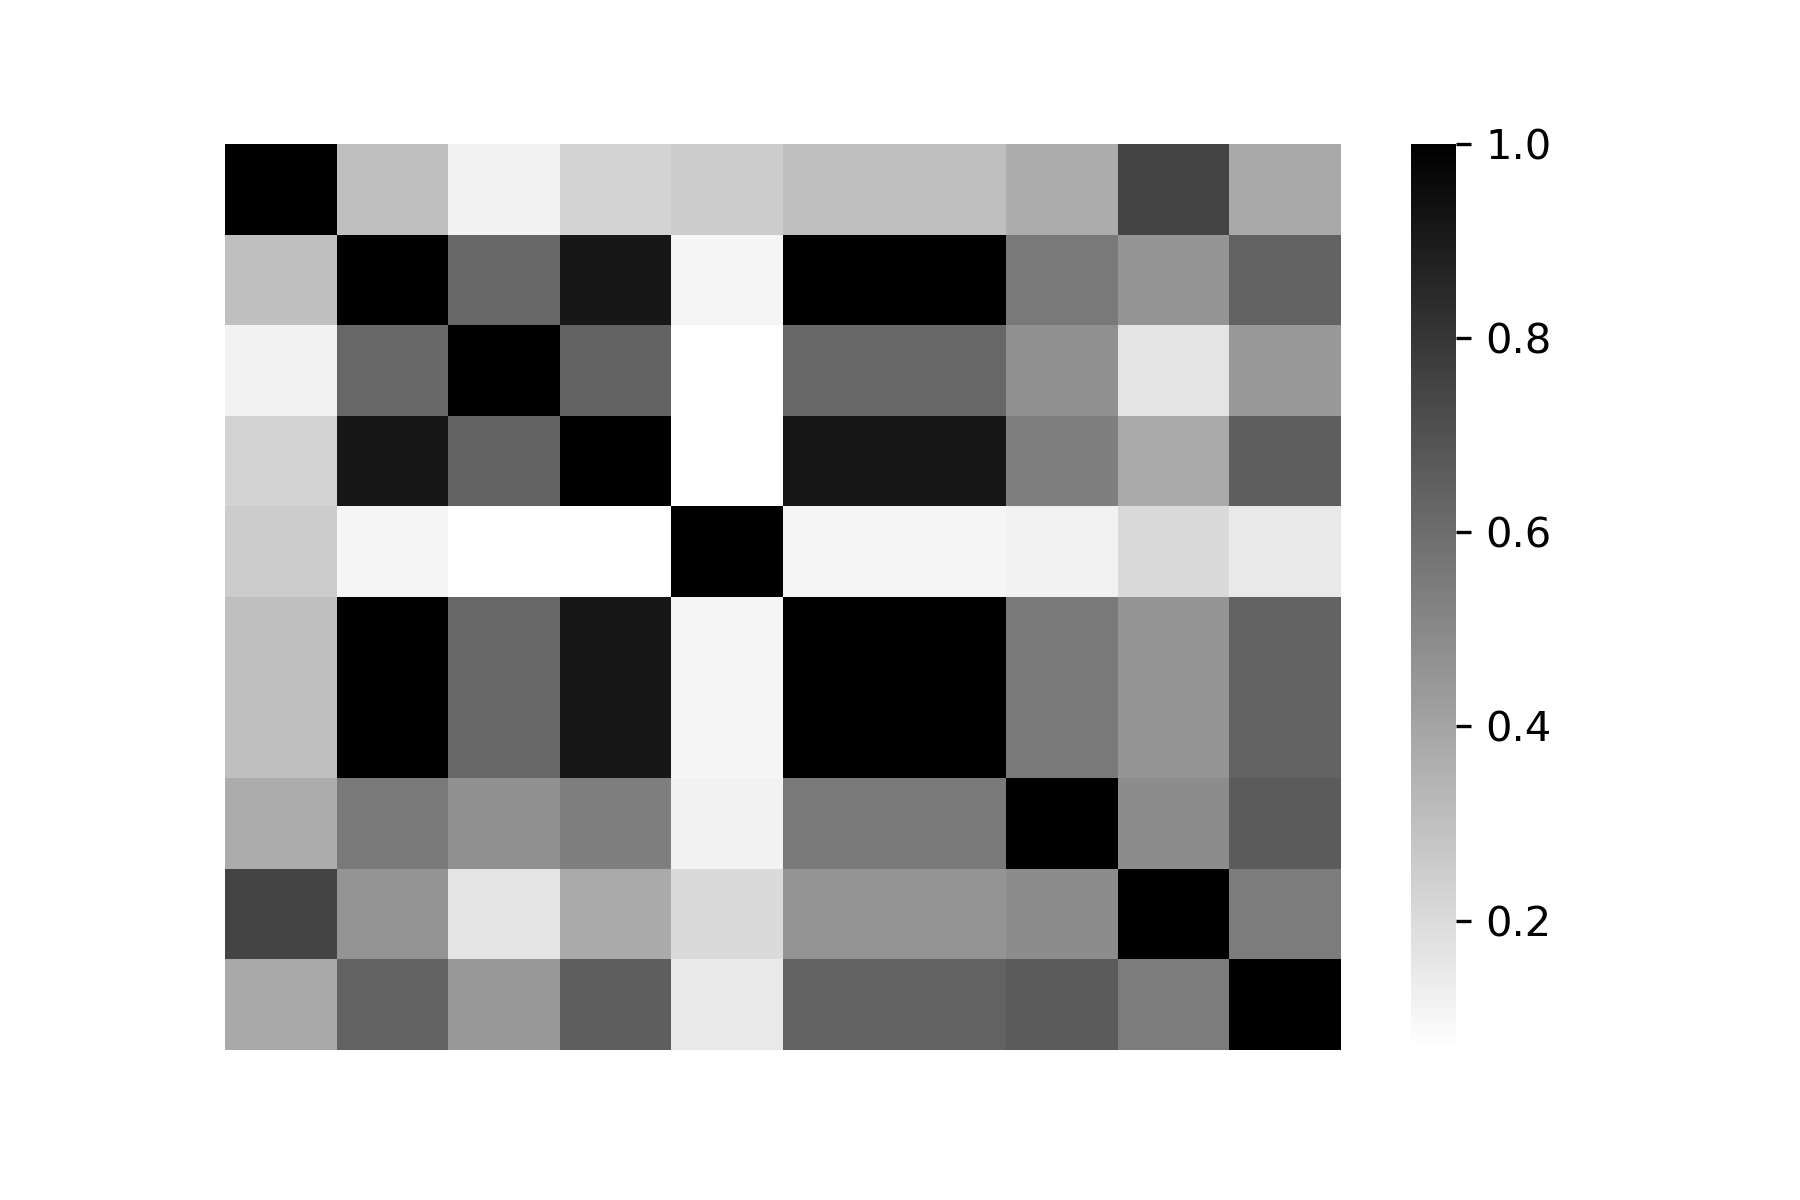
\includegraphics[scale=0.41]{images/results/MAP_1275_SCBM_S_0.3_PRECISION}}
\hspace{-1.5cm}
\subfloat[Greedy-String-Tiling]{
\label{GST_set_A}
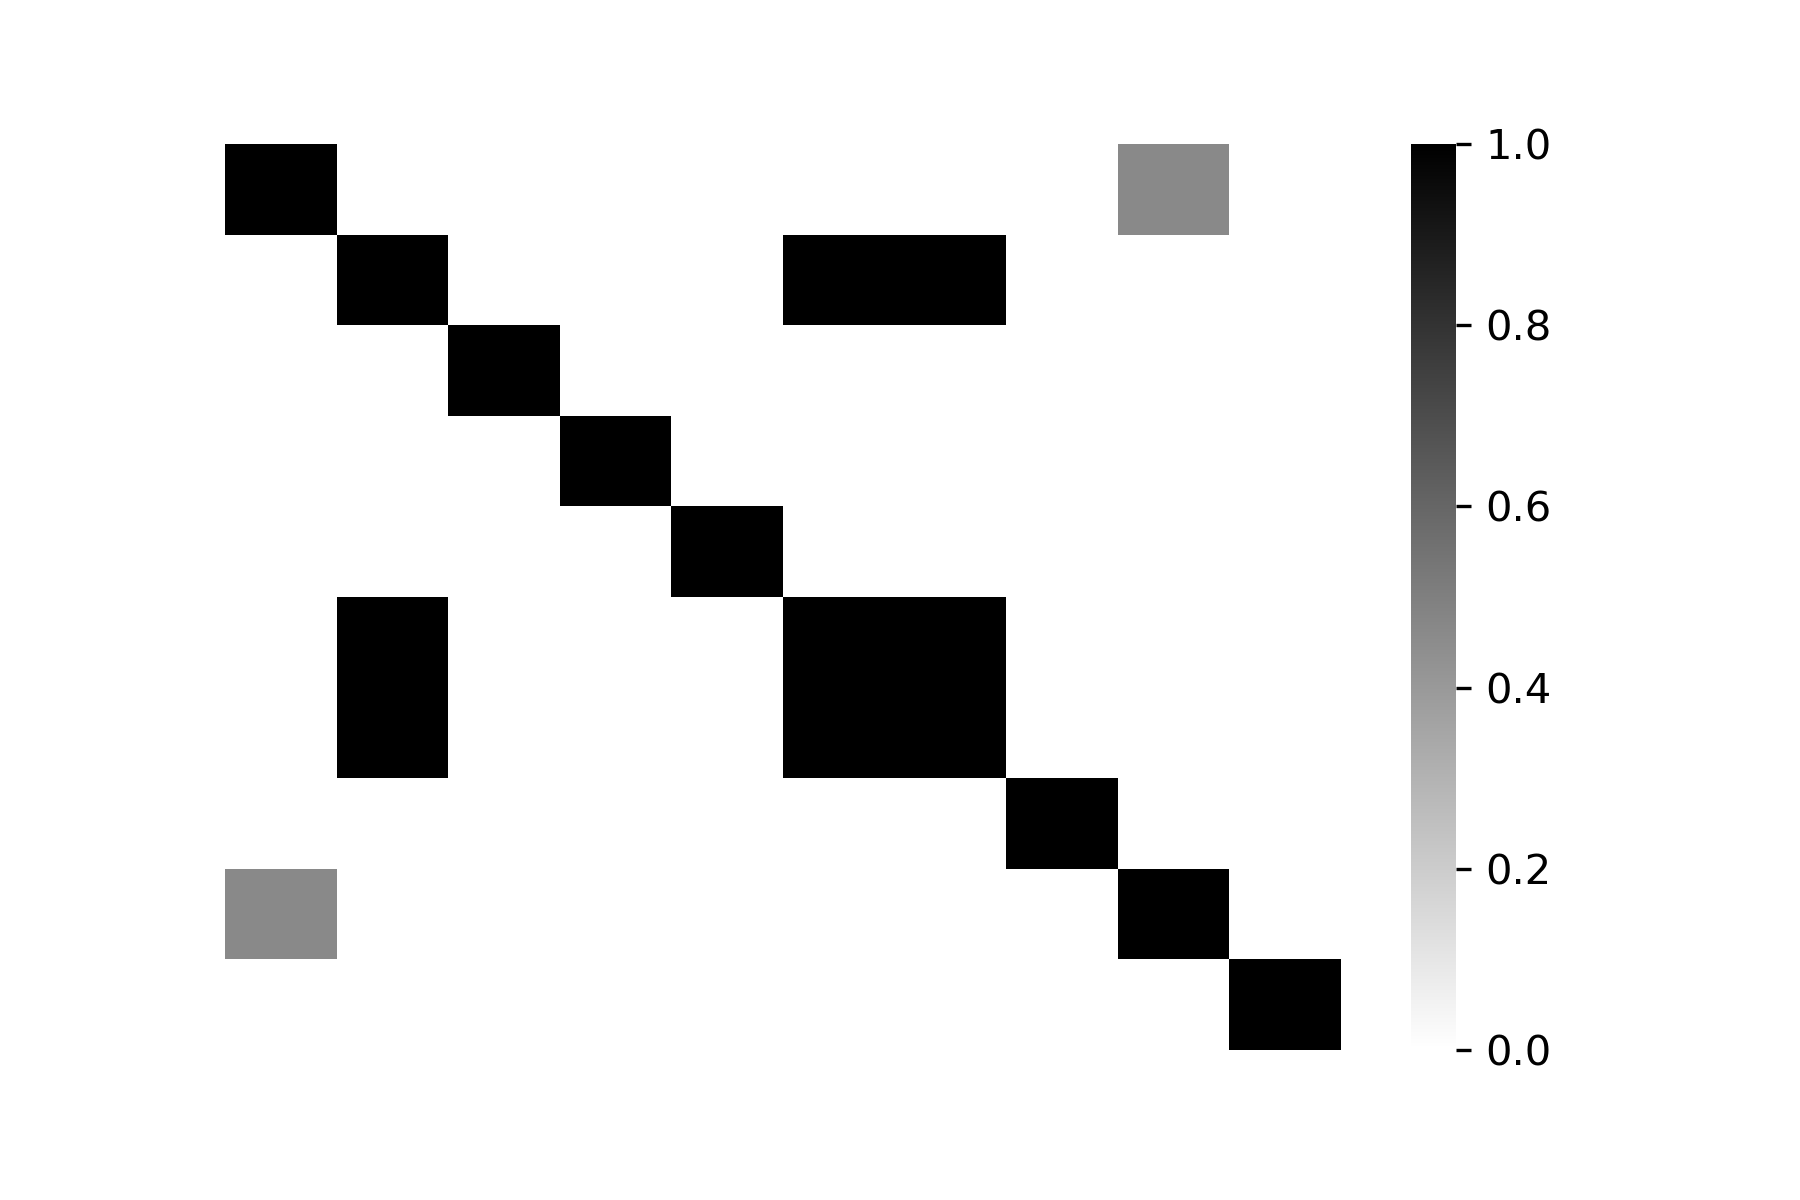
\includegraphics[scale=0.41]{images/results/MAP_1275_RKRGST_T_30_PRECISION}}
\hspace{-1.5cm}
\subfloat[Winnowing-Fingerprint]{
\label{WIN_set_A}
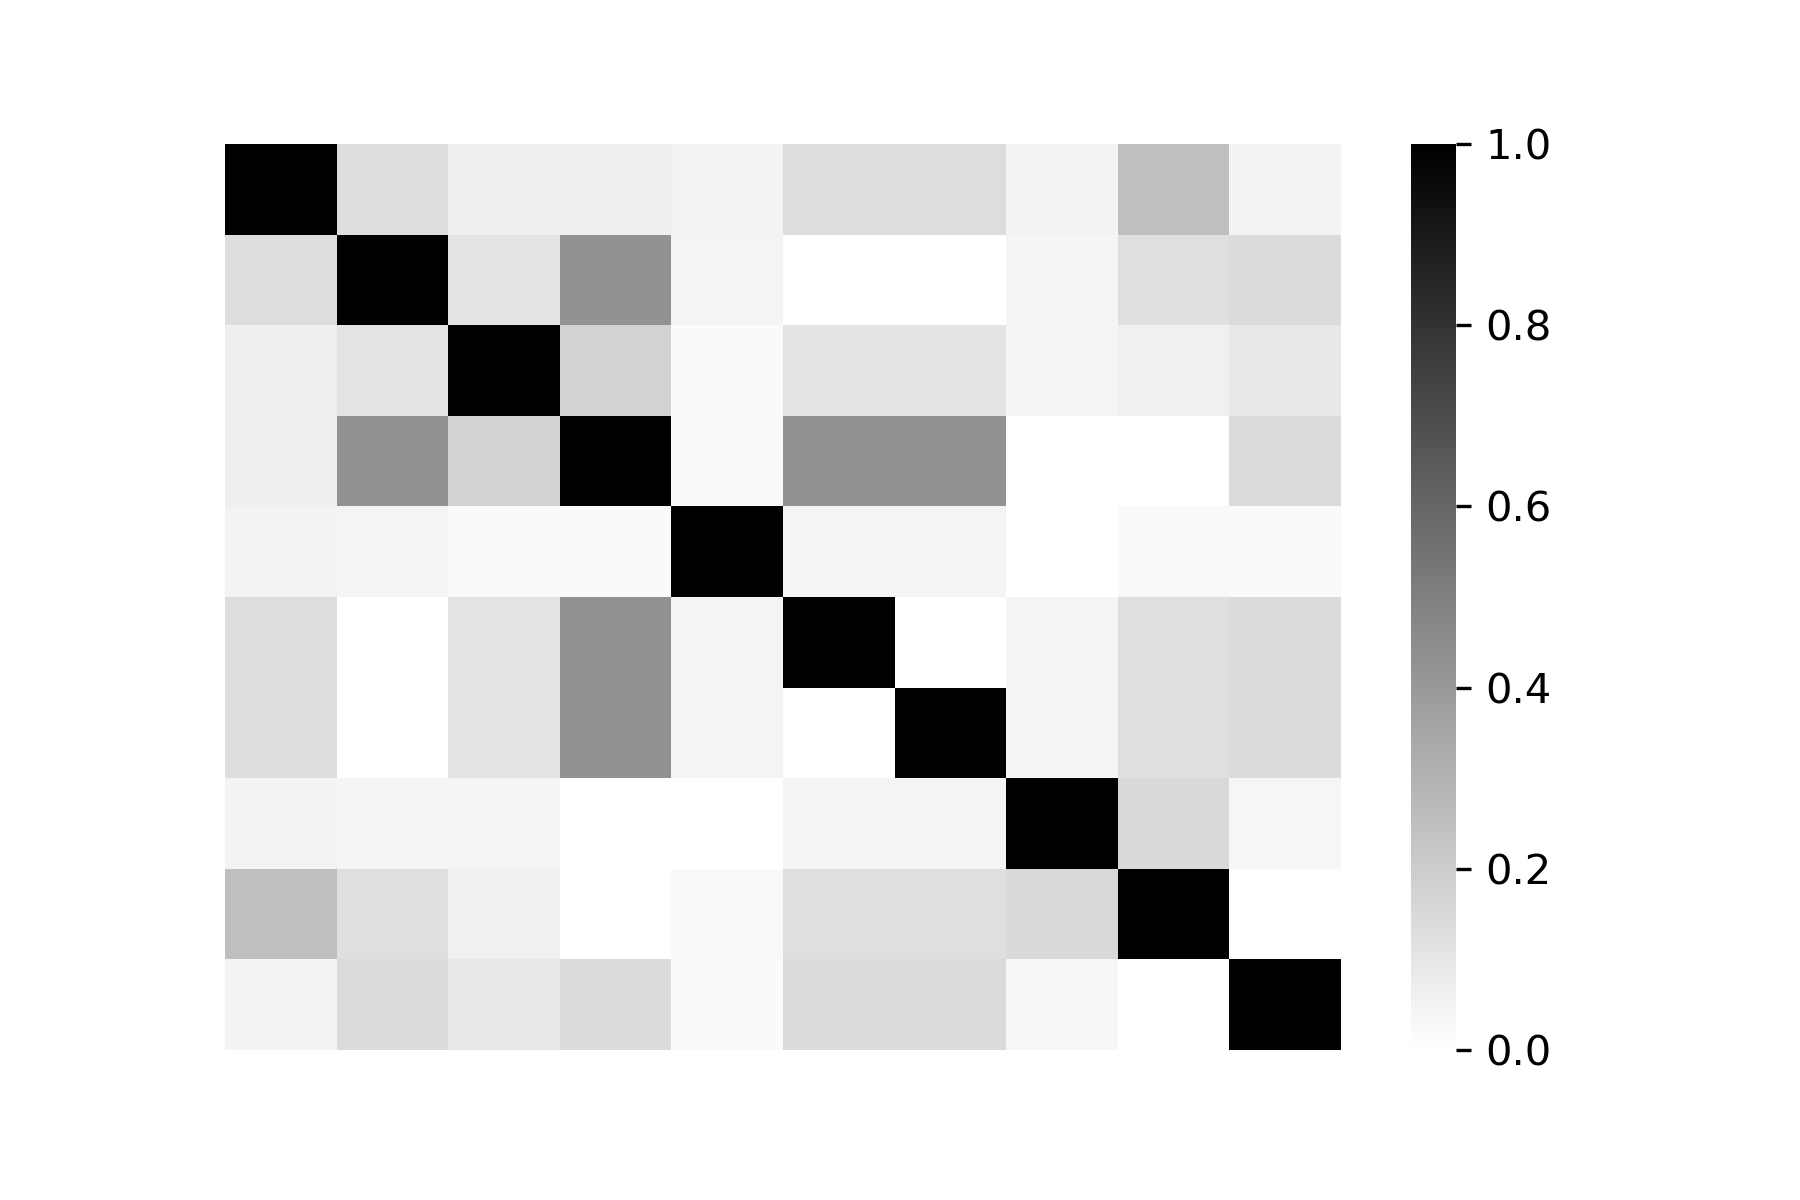
\includegraphics[scale=0.41]{images/results/MAP_1275_WIN_W_15_K_5_PRECISION}}
\caption{Prueba precisión I, conjunto A}
Fuente: Elaboración propia.
\label{set_A_precision}
\end{figure}

\subsubsection{Conjunto B}
La matriz de similitud que se obtuvo para este conjunto de prueba. Se muestra que empiezan a notarse la diferencia respecto a la precisión de los algoritmos, SCBM obtiene mas casos positivos de similitud que Winnowing.
\begin{figure}[!h]
\centering
\subfloat[SCBM]{
\label{SCBM_set_B}
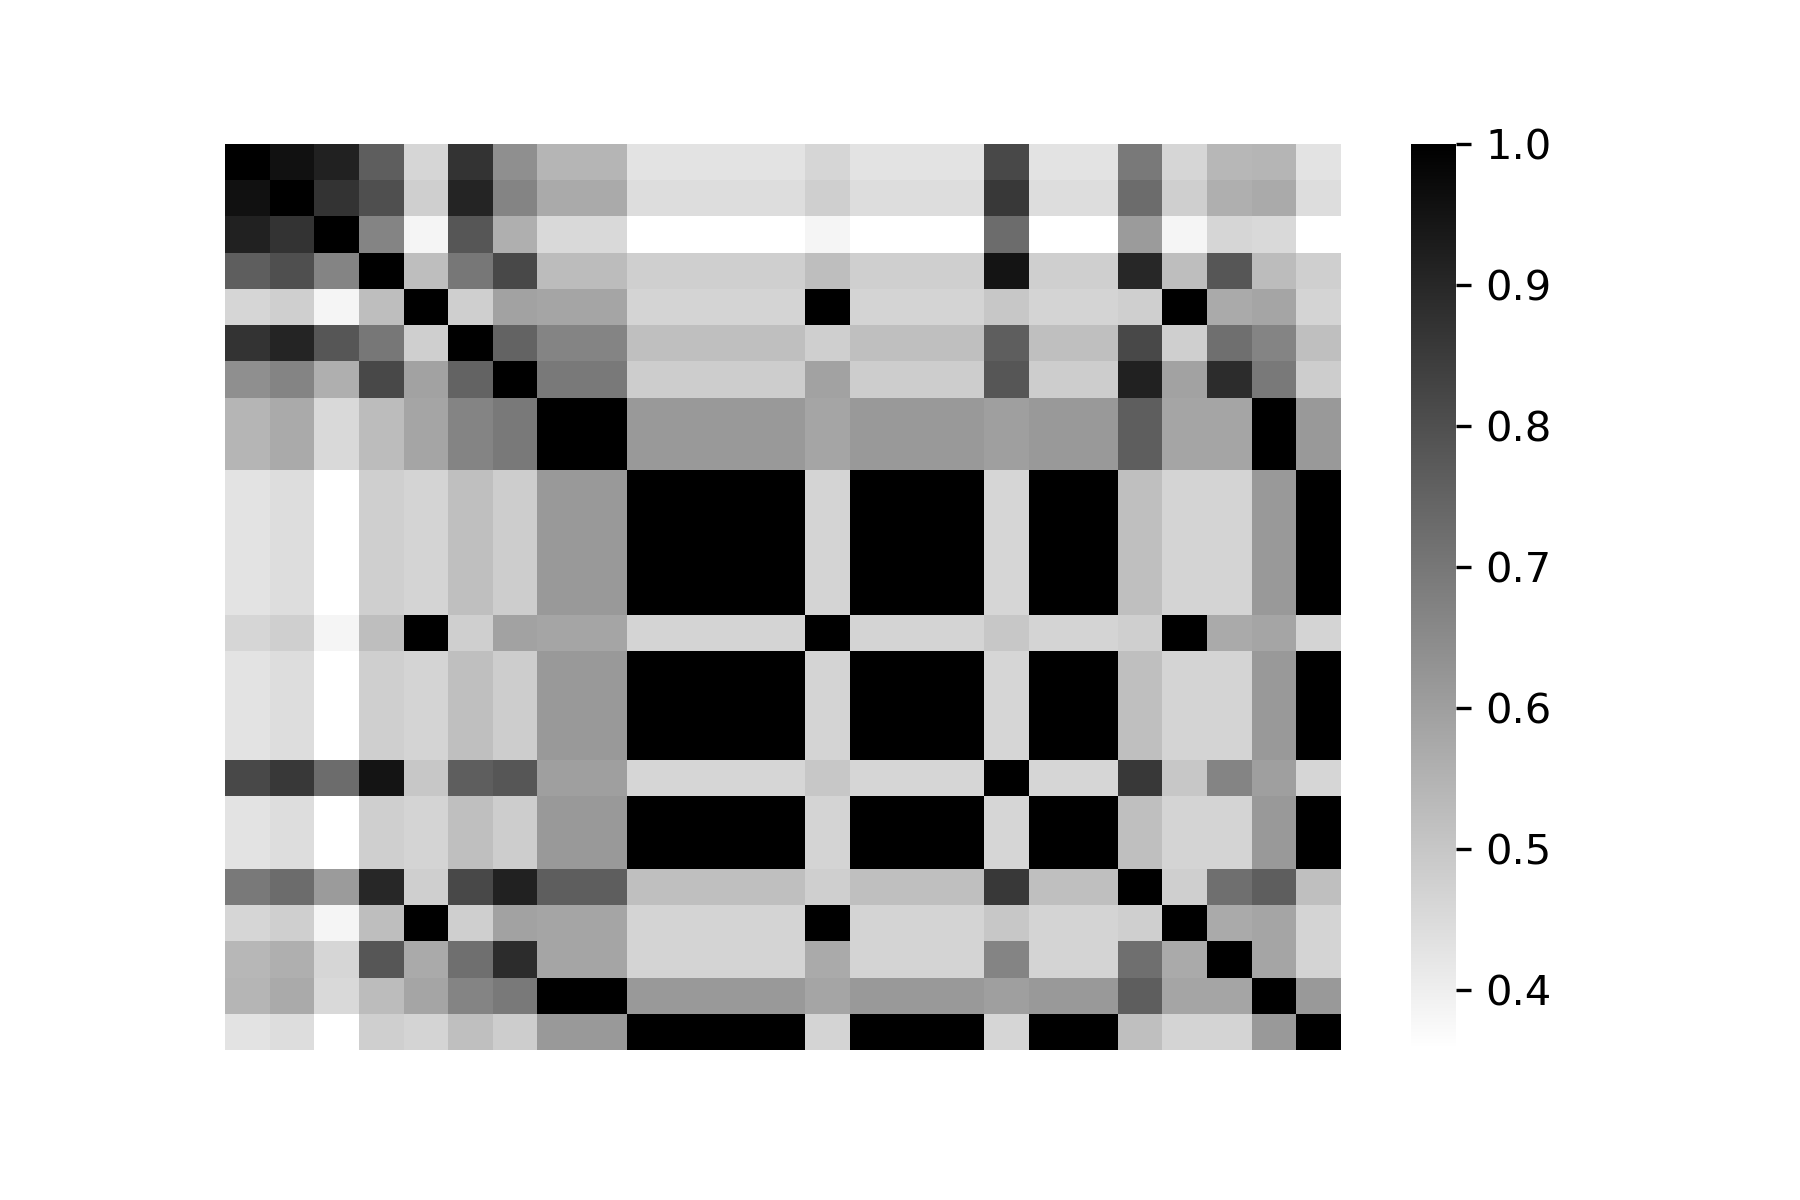
\includegraphics[scale=0.41]{images/results/MAP_1407_SCBM_S_0.3_PRECISION}}
\hspace{-1.5cm}
\subfloat[Greedy-String-Tiling]{
\label{GST_set_B}
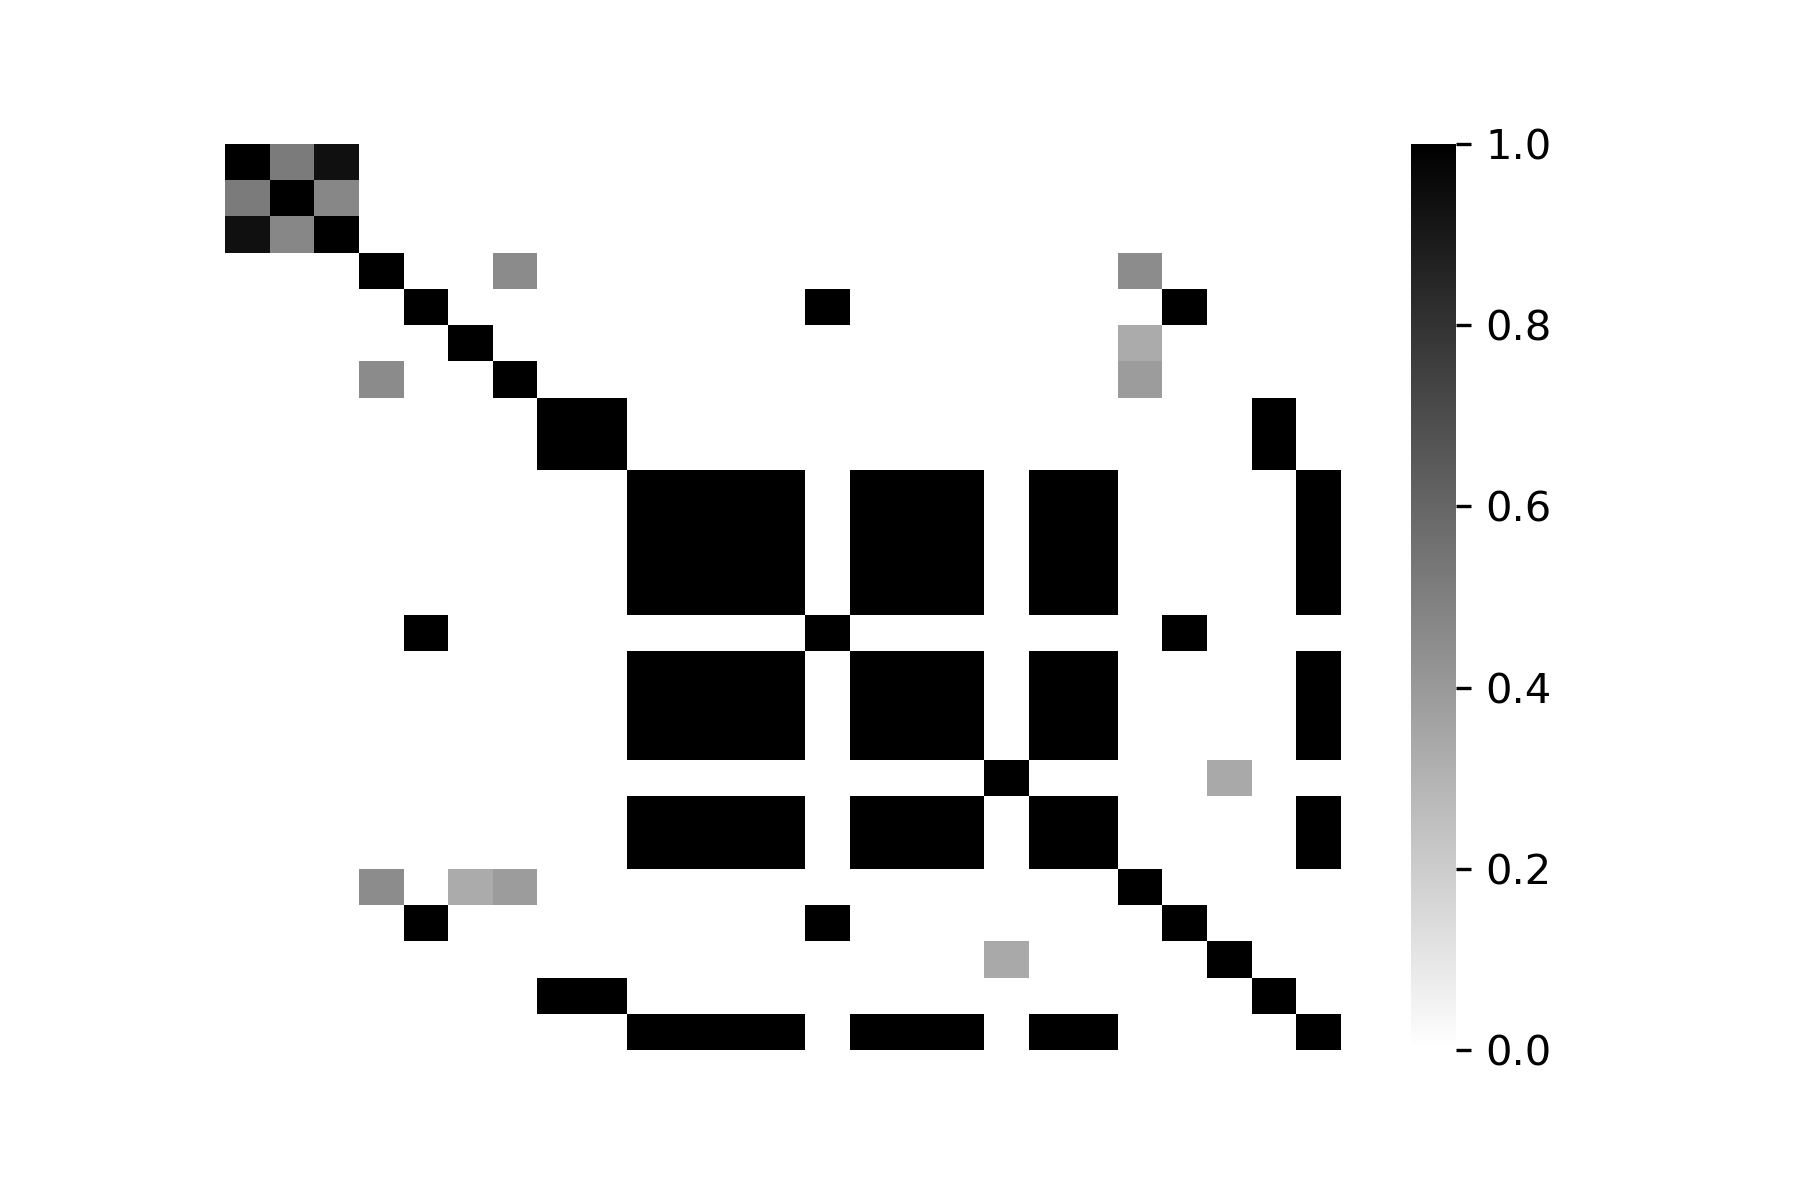
\includegraphics[scale=0.41]{images/results/MAP_1407_RKRGST_T_30_PRECISION}}
\hspace{-1.5cm}
\subfloat[Winnowing-Fingerprint]{
\label{WIN_set_B}
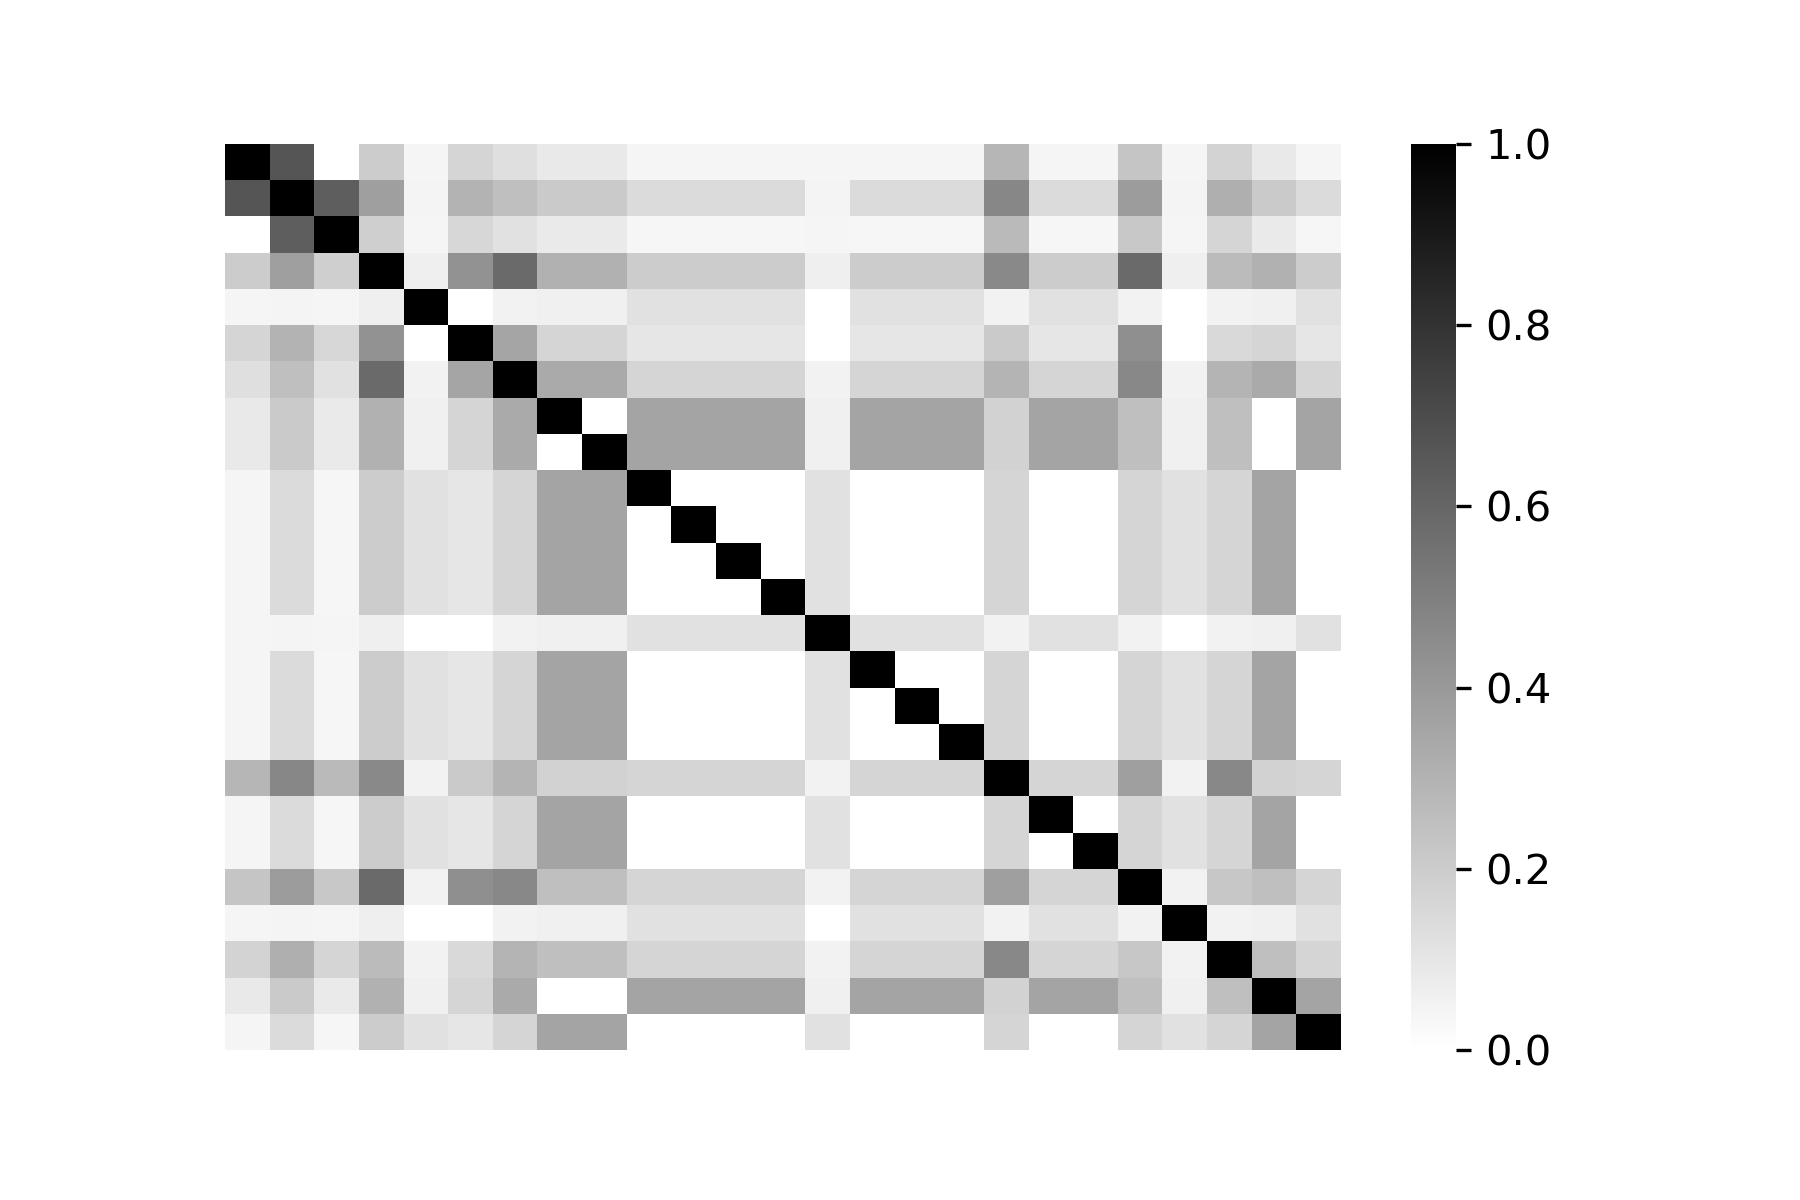
\includegraphics[scale=0.41]{images/results/MAP_1407_WIN_W_15_K_5_PRECISION}}
\caption{Prueba precisión I, conjunto B}
Fuente: Elaboración propia.
\label{set_B_precision}
\end{figure}
\subsubsection{Conjunto C}
La matriz de similitud que se obtuvo para este conjunto de prueba. Continua la diferencia respecto a la precisión de los algoritmos, SCBM obtiene mas casos positivos de similitud que Winnowing.
\begin{figure}[!h]
\centering
\subfloat[SCBM]{
\label{SCBM_set_C}
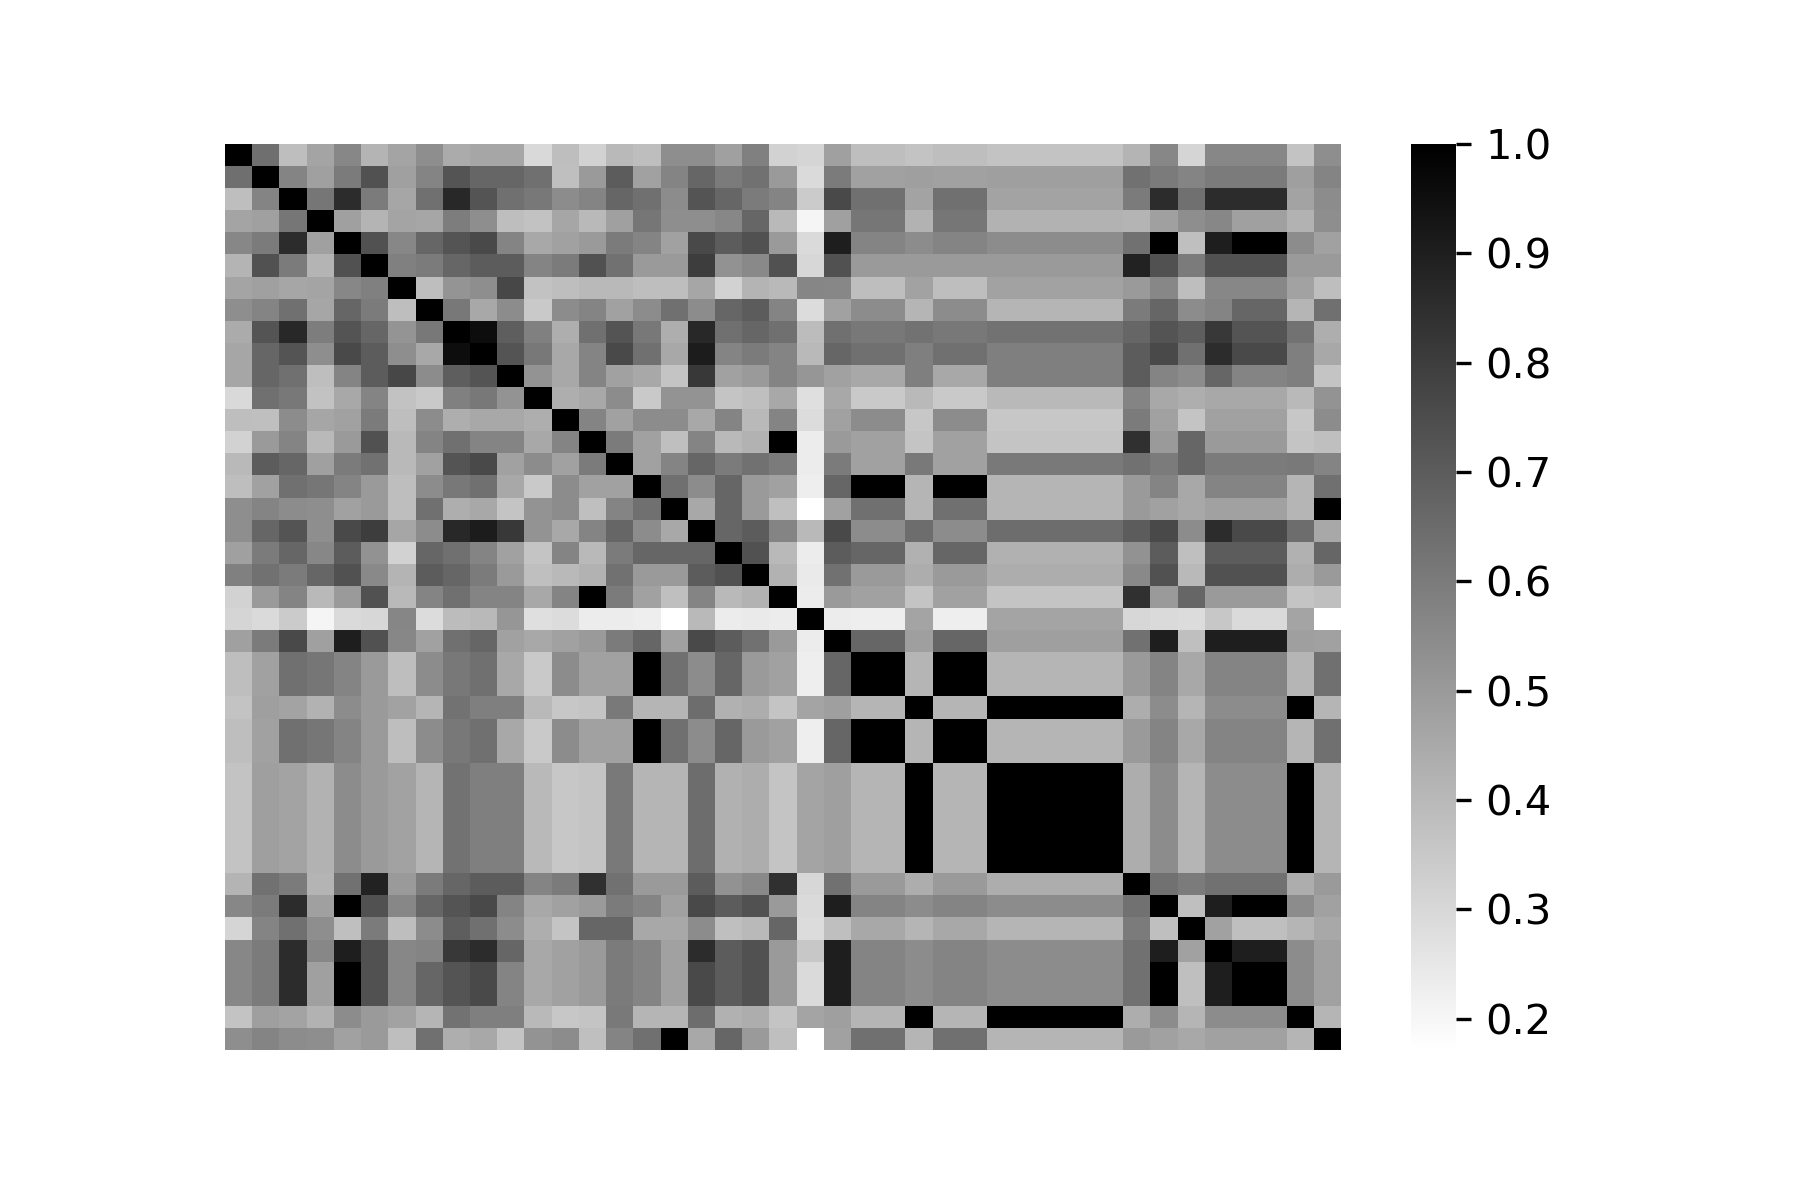
\includegraphics[scale=0.41]{images/results/MAP_1588_SCBM_S_0.3_PRECISION}}
\hspace{-1.5cm}
\subfloat[Greedy-String-Tiling]{
\label{GST_set_C}
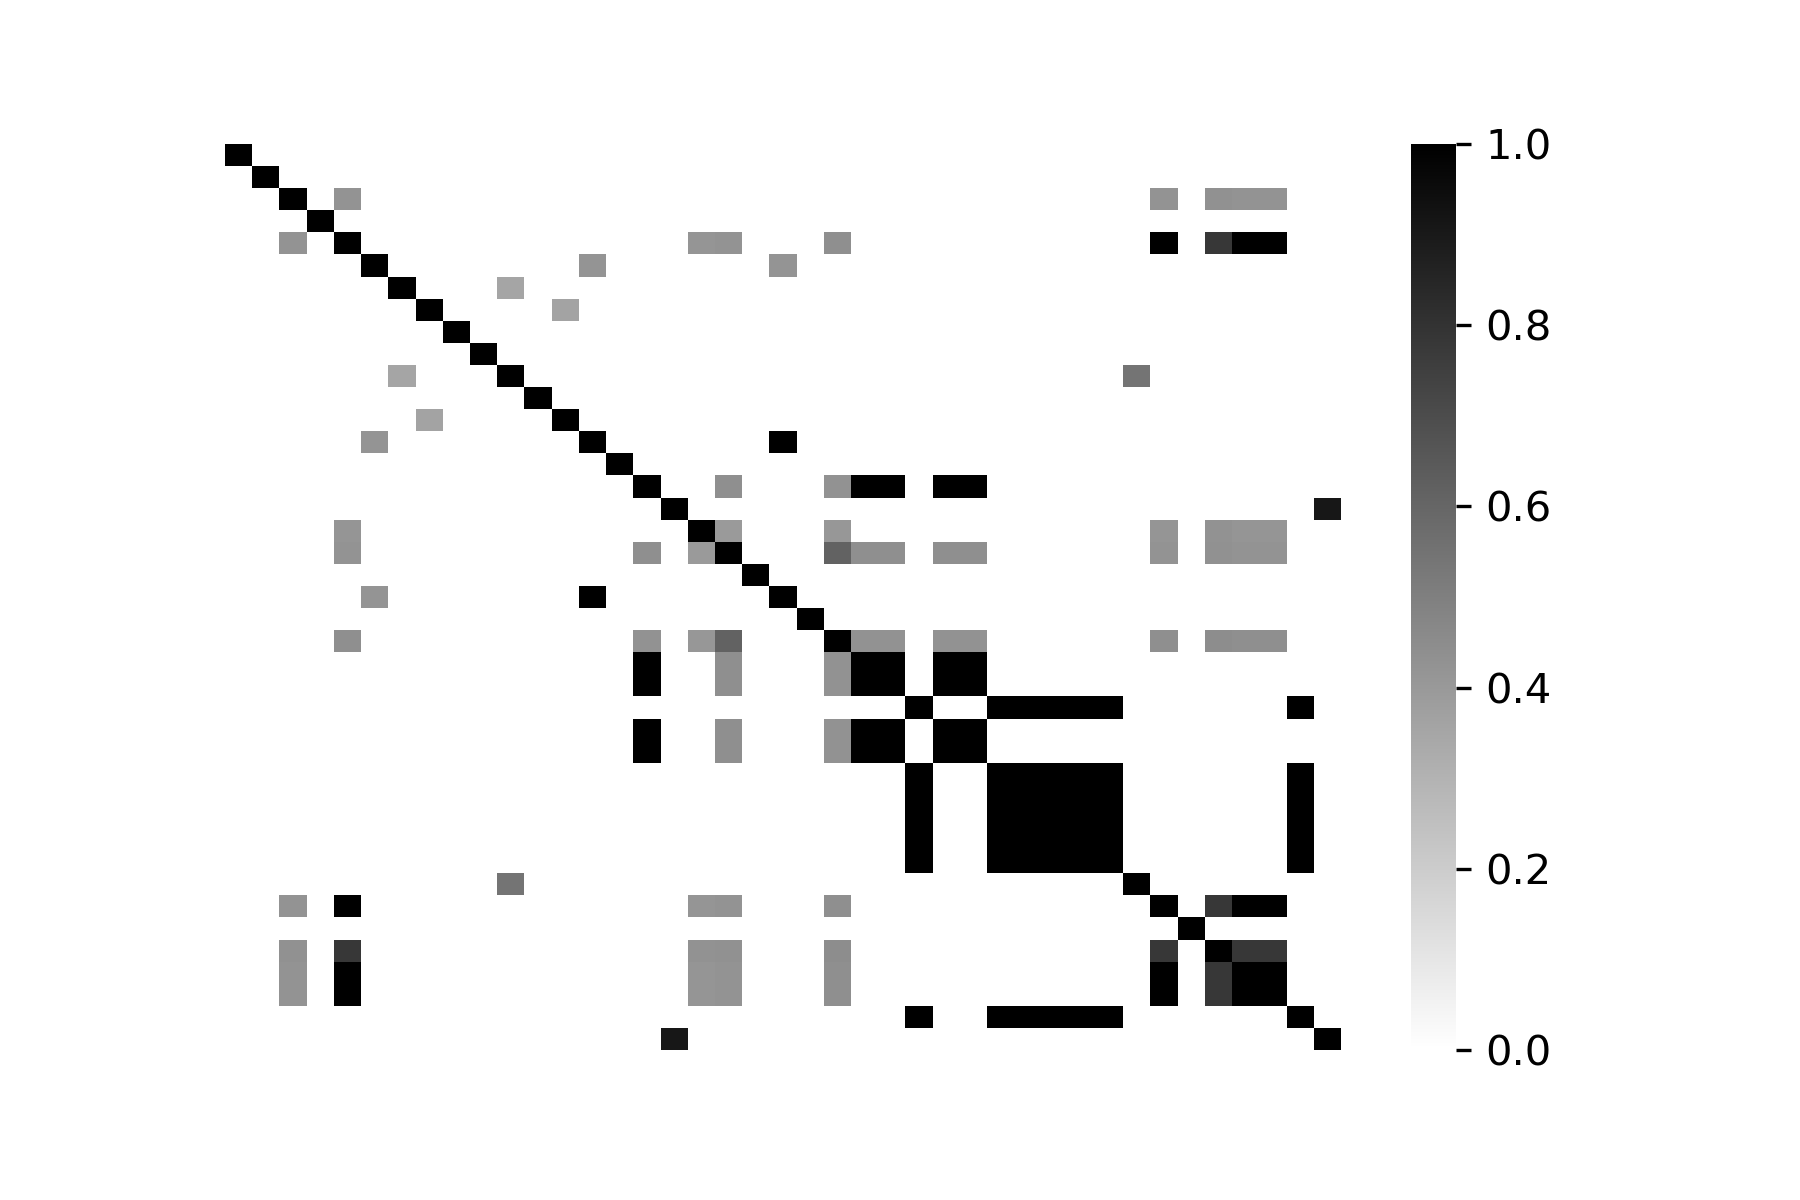
\includegraphics[scale=0.41]{images/results/MAP_1588_RKRGST_T_30_PRECISION}}
\hspace{-1.5cm}
\subfloat[Winnowing-Fingerprint]{
\label{WIN_set_C}
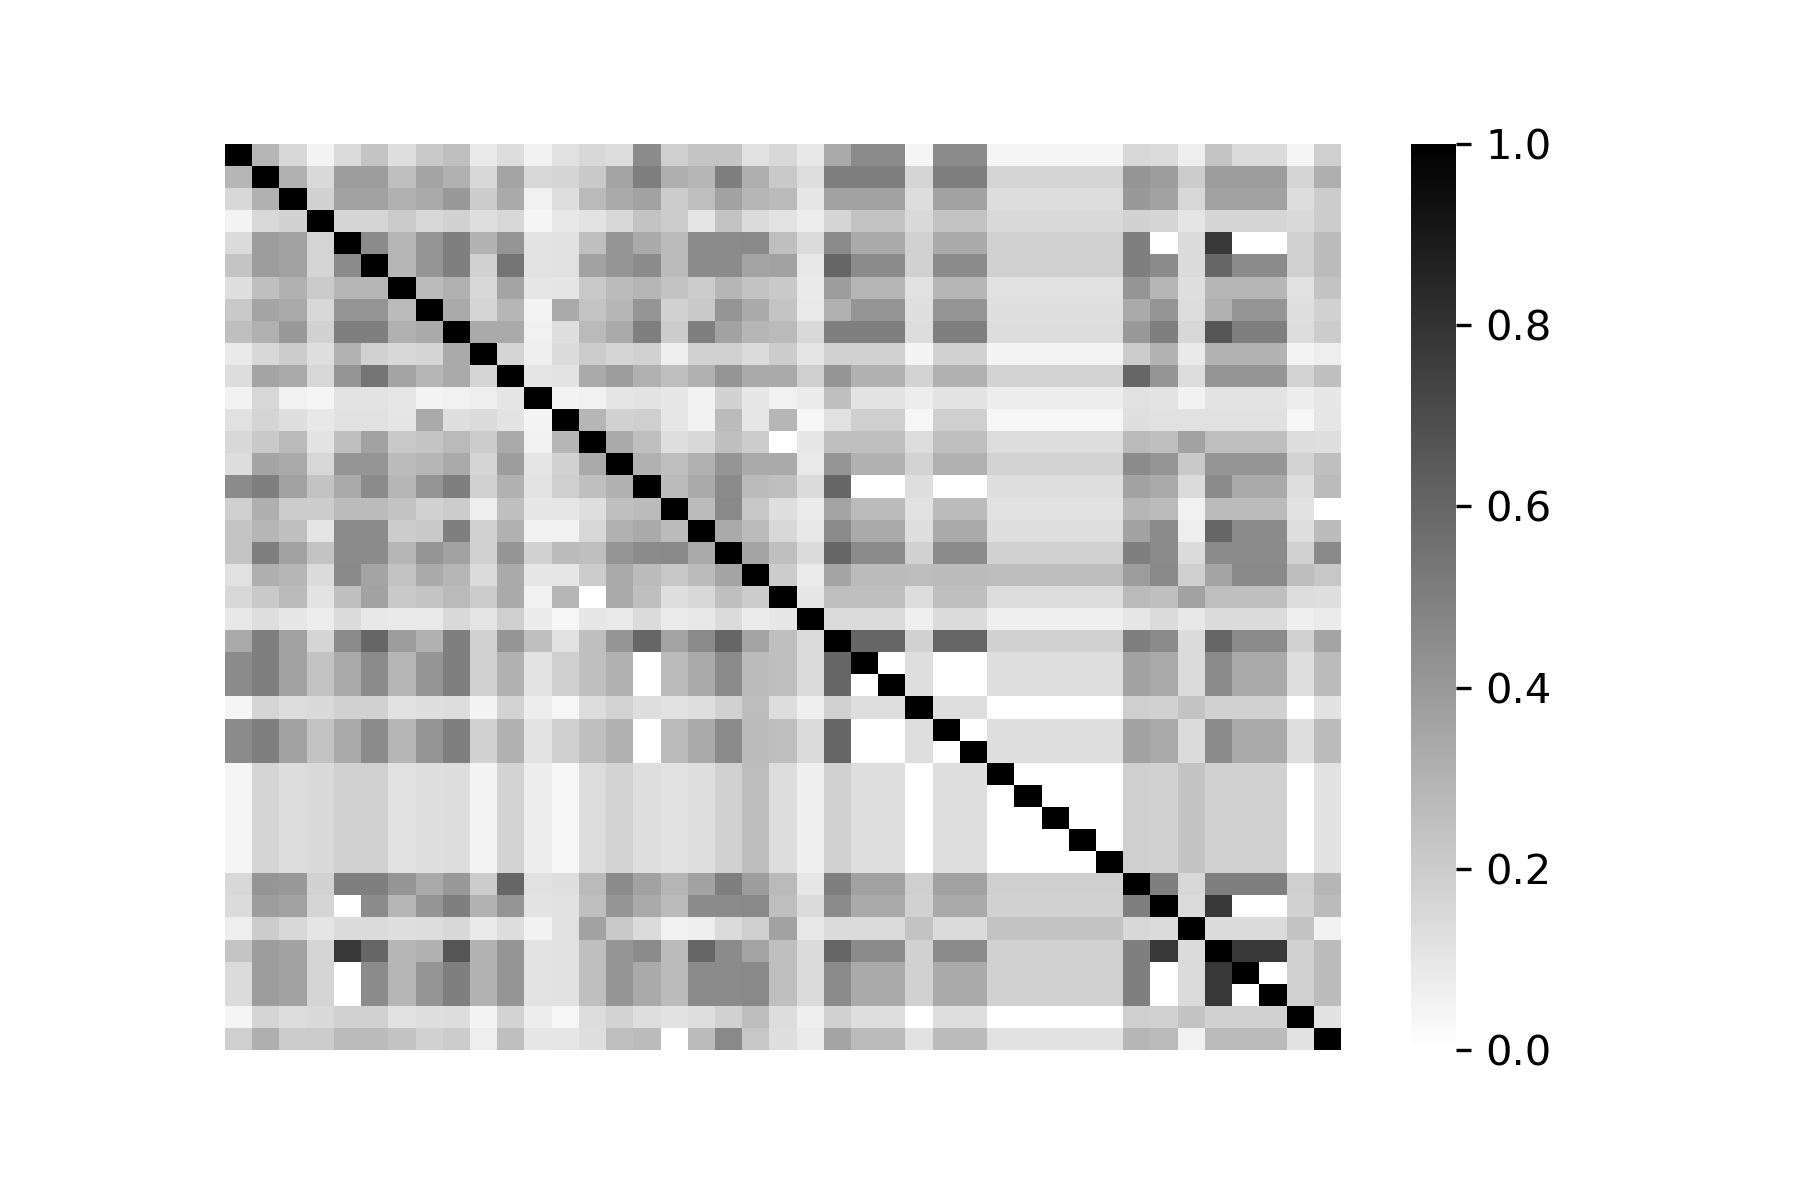
\includegraphics[scale=0.41]{images/results/MAP_1588_WIN_W_15_K_5_PRECISION}}
\caption{Prueba precisión I, conjunto C}
Fuente: Elaboración propia.
\label{set_C_precision}
\end{figure}
\subsubsection{Conjunto D}
La matriz de similitud que se obtuvo para este conjunto de prueba. Continua la diferencia respecto a la precisión de los algoritmos, SCBM obtiene un casos en el que no logra identificar la similitud mientras Winnowing si logra identificarlos.
\begin{figure}[!h]
\centering
\subfloat[SCBM]{
\label{SCBM_set_D}
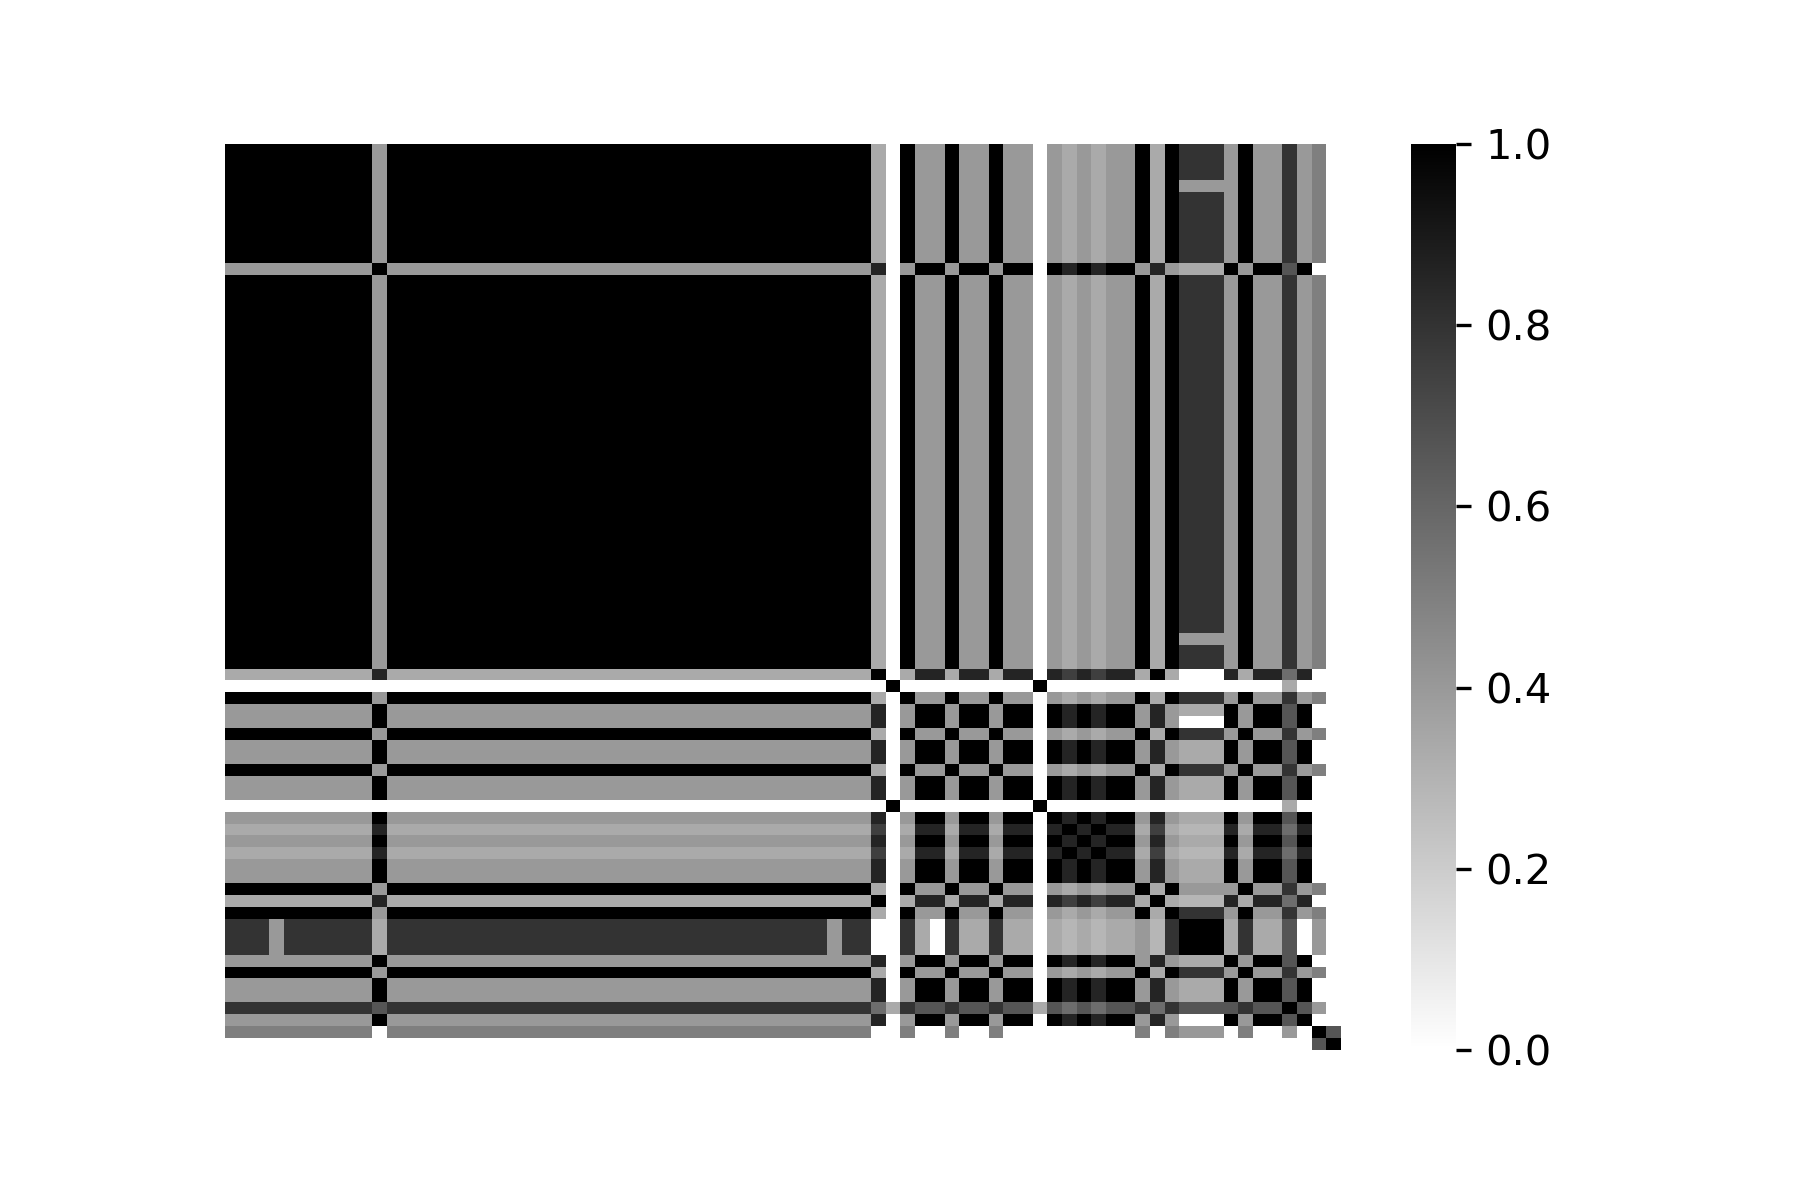
\includegraphics[scale=0.41]{images/results/MAP_1222_SCBM_S_0.3_PRECISION}}
\hspace{-1.5cm}
\subfloat[Greedy-String-Tiling]{
\label{GST_set_D}
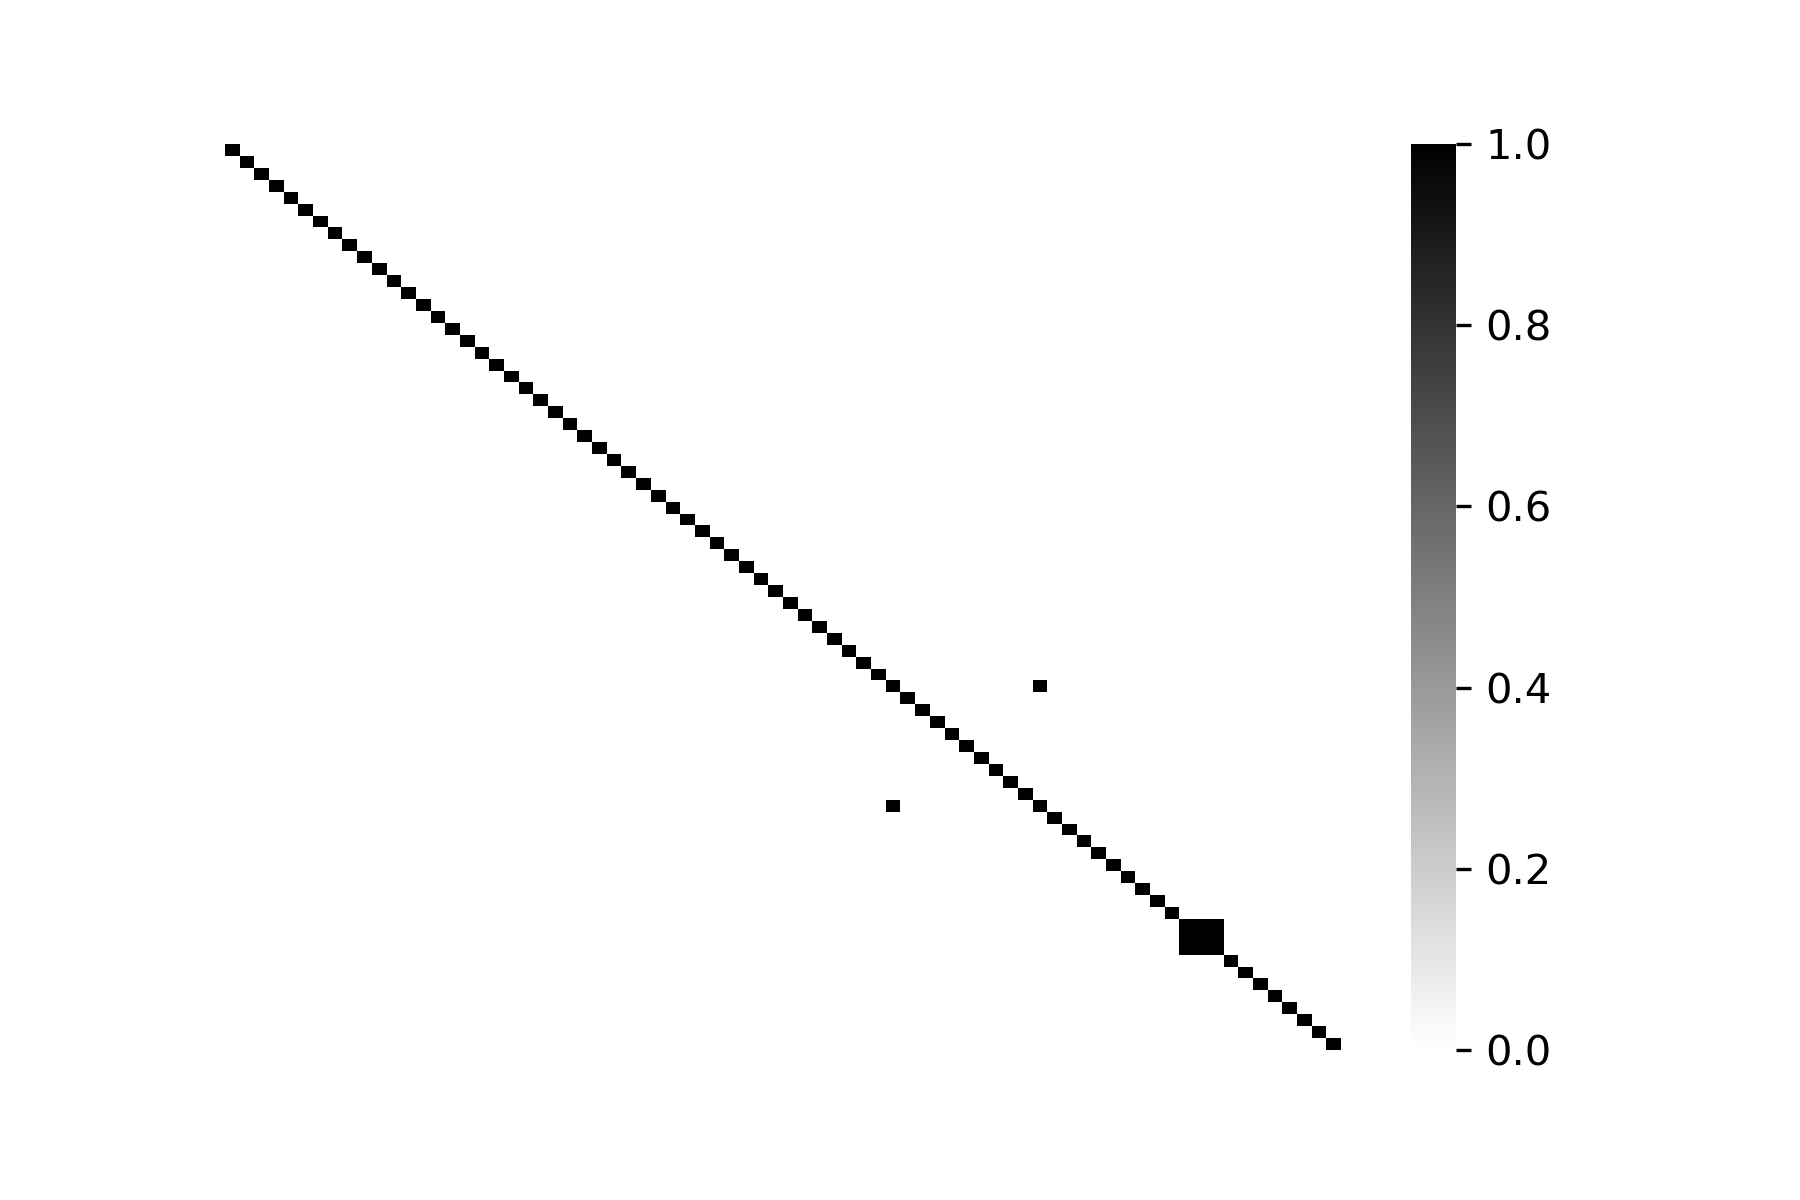
\includegraphics[scale=0.41]{images/results/MAP_1222_RKRGST_T_30_PRECISION}}
\hspace{-1.5cm}
\subfloat[Winnowing-Fingerprint]{
\label{WIN_set_D}
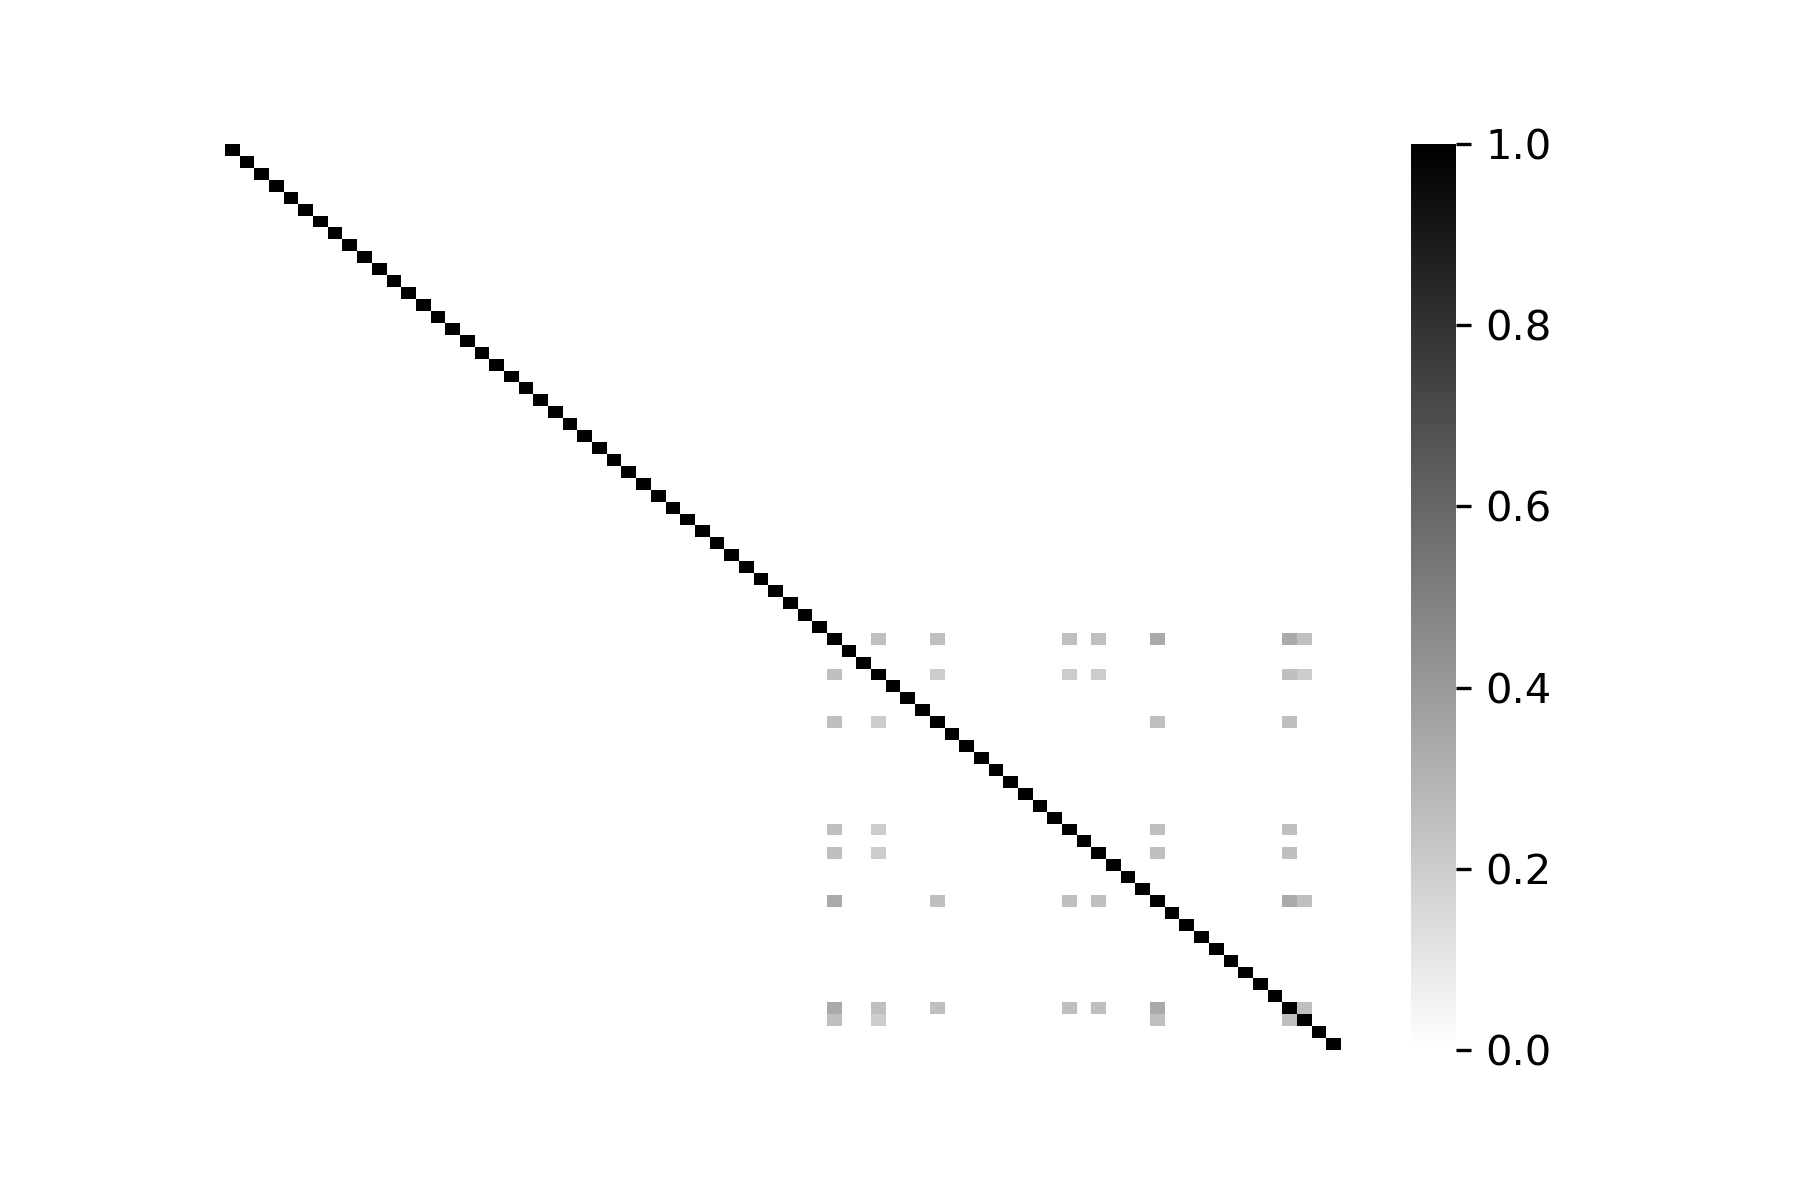
\includegraphics[scale=0.41]{images/results/MAP_1222_WIN_W_15_K_5_PRECISION}}
\caption{Prueba precisión I, conjunto D}
Fuente: Elaboración propia.
\label{set_D_precision}
\end{figure}
\subsubsection{Conjunto E}
La matriz de similitud que se obtuvo para este conjunto de prueba. Continua la diferencia respecto a la precisión de los algoritmos, SCBM obtiene un casos en el que no logra identificar la similitud mientras Winnowing si logra identificarlos.
\begin{figure}[!h]
\centering
\subfloat[SCBM]{
\label{SCBM_set_E}
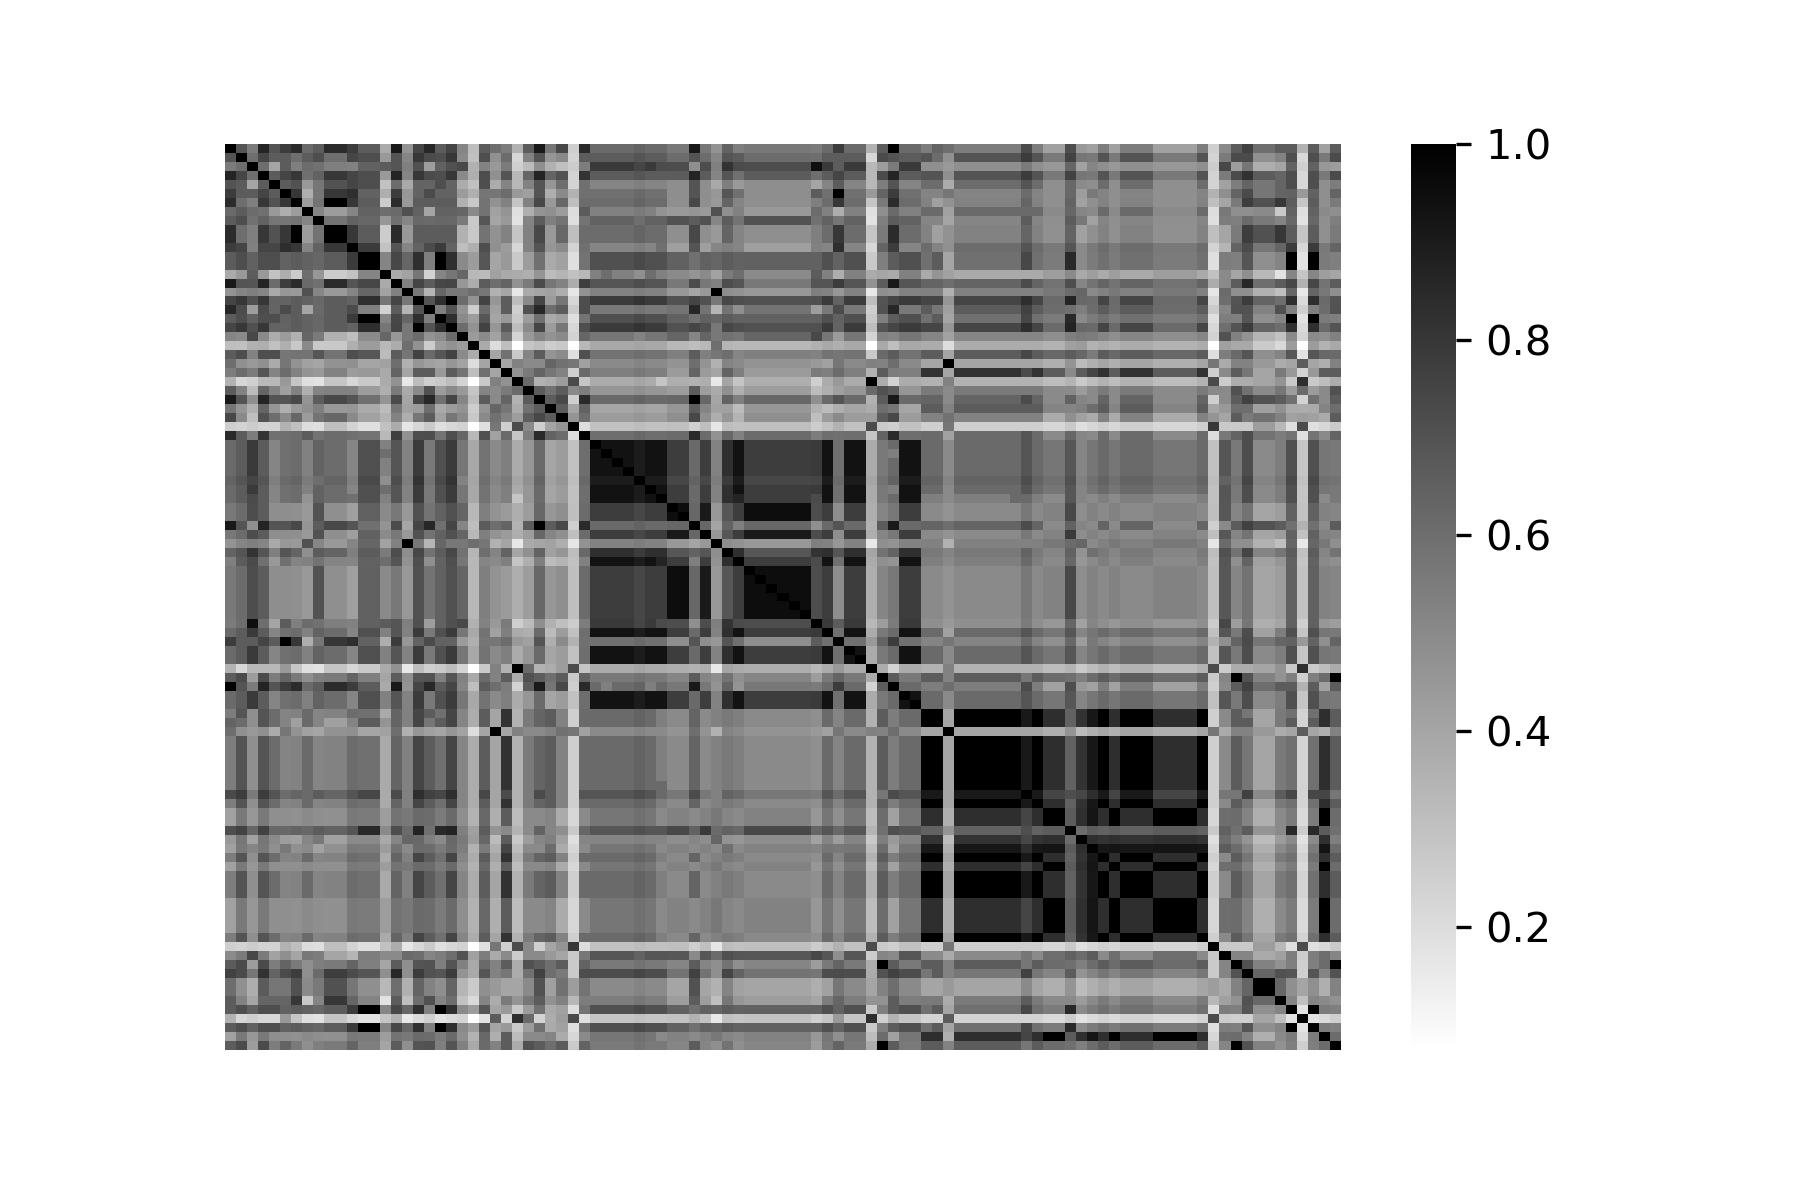
\includegraphics[scale=0.41]{images/results/MAP_1089_SCBM_S_0.3_PRECISION}}
\hspace{-1.5cm}
\subfloat[Greedy-String-Tiling]{
\label{GST_set_E}
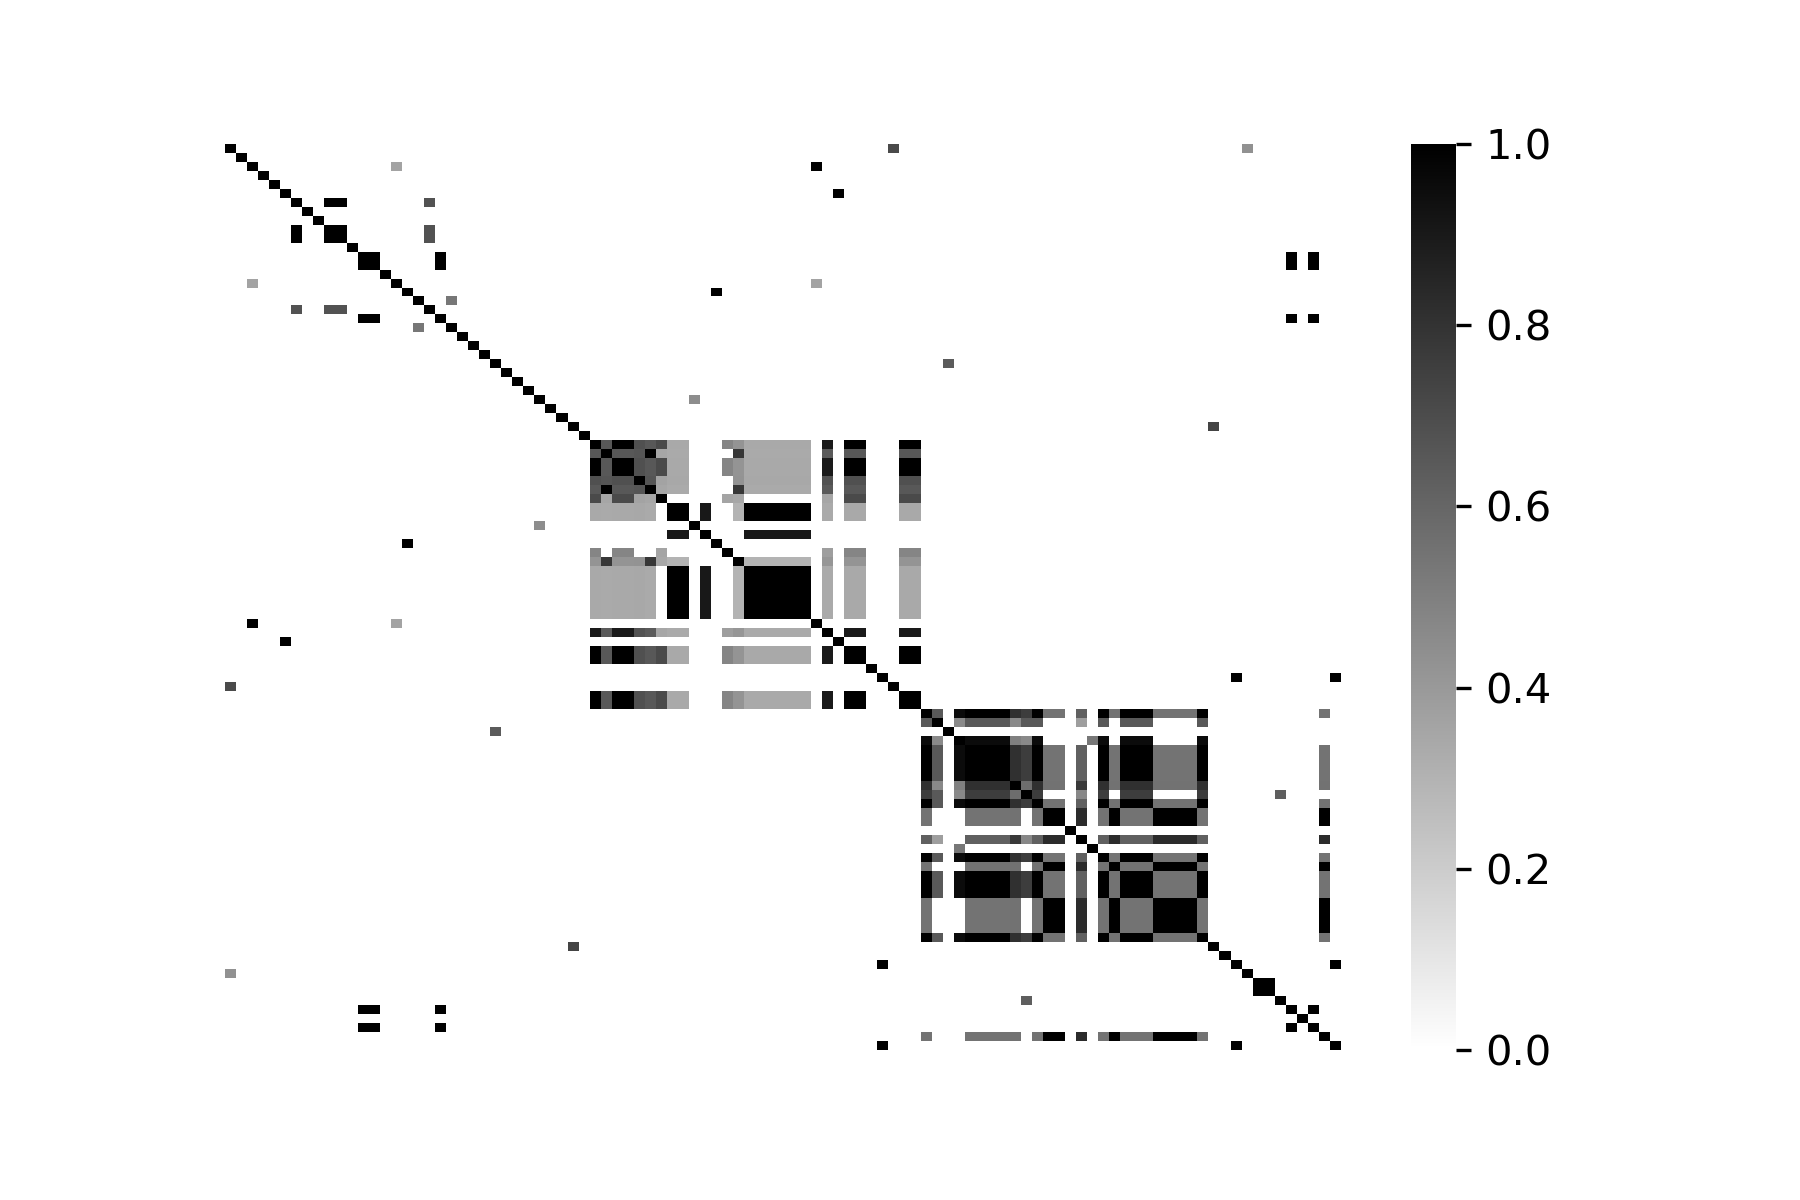
\includegraphics[scale=0.41]{images/results/MAP_1089_RKRGST_T_30_PRECISION}}
\hspace{-1.5cm}
\subfloat[Winnowing-Fingerprint]{
\label{WIN_set_E}
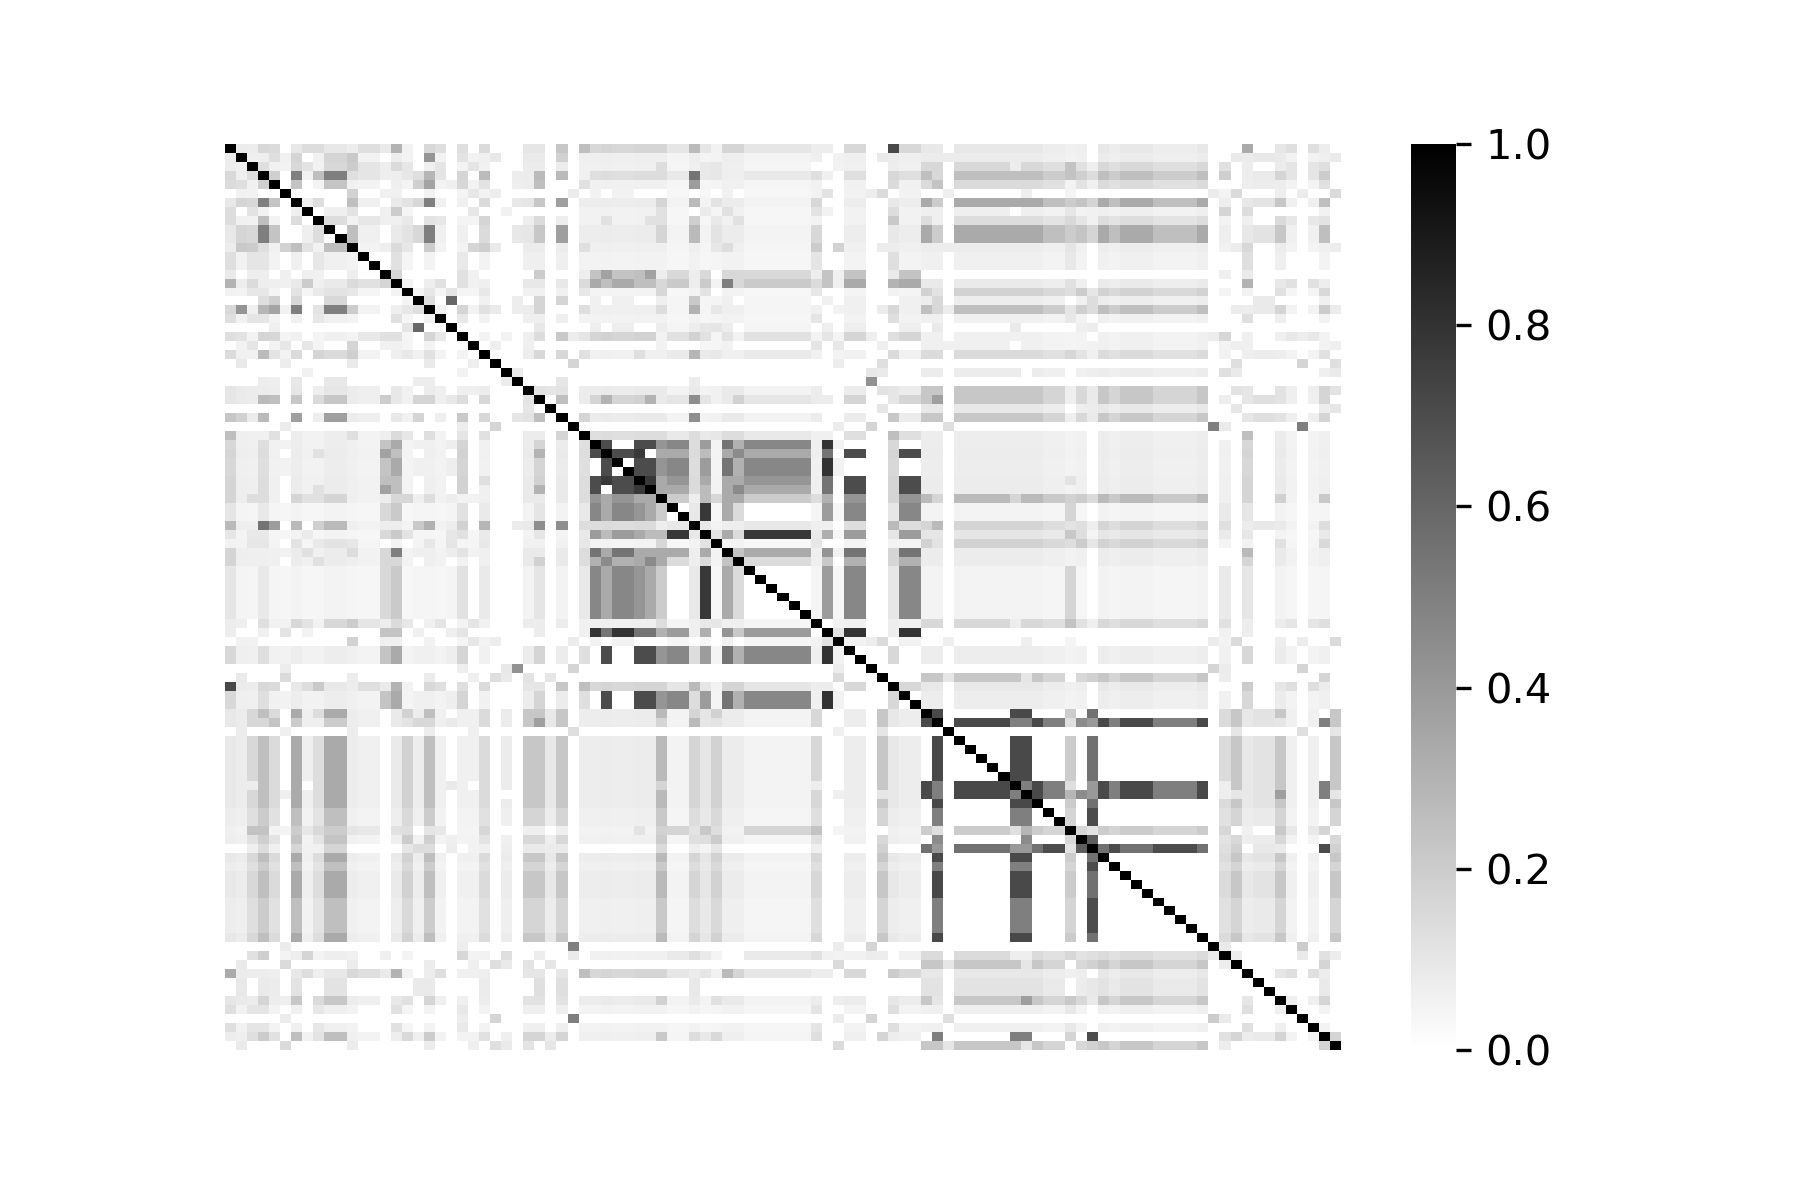
\includegraphics[scale=0.41]{images/results/MAP_1089_WIN_W_15_K_5_PRECISION}}
\caption{Prueba precisión I, conjunto E}
Fuente: Elaboración propia.
\label{set_E_precision}
\end{figure}

\subsection{Tiempo de ejecución de la prueba I}
En la tabla \ref{pruebaTiempo} se presentan los resultados obtenidos, respecto al tiempo de ejecucion de cada algoritmo al calcular la similitud de cada conjunto de prueba. Los resultados obtenidos se encuentran en segundos.

\begin{table}[H]
\centering
\begin{tabular}{|c||c||c||c|}
\hline
Conjunto & SCBM & Greedy-String-Tiling & Winnowing-Fingerprint \\ \hline
A & 11.77 seg.  & 0.86 seg. &1  \\ \hline
B & 4.16 seg.  & 3.66 seg. &2 \\ \hline
C & 14.53 seg.  & 12.73 seg. &3  \\ \hline
D & 3.28 seg.  & 19.47 seg. &4 \\ \hline
E & 52.00 seg.  & 42.73 seg. &5 \\ \hline
\end{tabular}
\caption{Detalle del promedio de tiempo de ejecución de los algoritmos.}
Fuente: Elaboración propia.
\label{pruebaTiempo}
\end{table}


\begin{itemize}
  \item Con las prueba realizada demuestro que el algoritmo de Winnowing es mejor por segundos respecto al tiempo de ejecución. El algoritmo SCBM presenta mejores resultados comparando archivos de codigo fuente que no tengan muchas instruciones.
\end{itemize}
